%%%%%%%%%%%%%%%%%%%%%%%%%%%%%%%%%%%%%%%%%%%%%%%%%%%%%%%%%%%%%%%%%%%%%%%%%%%%%%%%
%2345678901234567890123456789012345678901234567890123456789012345678901234567890
%        1         2         3         4         5         6         7         8

%\documentclass[letterpaper, 10 pt, conference]{ieeeconf}  % Comment this line out
                                                          % if you need a4paper


\documentclass[a4paper, 10pt, conference]{ieeeconf}      % Use this line for a4
                                     \usepackage[normalem]{ulem}                     % paper

\IEEEoverridecommandlockouts                              % This command is only
                                                          % needed if you want to
                                                          % use the \thanks command
\overrideIEEEmargins
% See the \addtolength command later in the file to balance the column lengths
% on the last page of the document


% !TEX root = ../main.tex
% !TeX encoding = UTF-8
\usepackage{verbatim}
\usepackage[portuguese]{babel}
%\usepackage[brazilian]{babel}
%\usepackage[brazilian]{babel}
\usepackage[utf8]{inputenc}
\usepackage[T1]{fontenc}


\usepackage{todonotes}
\usepackage[algoruled,linesnumbered,lined,portuguese]{algorithm2e}



\usepackage{tabularx}
\newcolumntype{L}[1]{>{\raggedright\arraybackslash}p{#1}}
\newcolumntype{C}[1]{>{\centering\arraybackslash}p{#1}}
\newcolumntype{R}[1]{>{\raggedleft\arraybackslash}p{#1}}

% *** CITATION PACKAGES ***
\usepackage{cite}


% *** GRAPHICS RELATED PACKAGES ***
%\usepackage[pdftex]{graphicx}

% *** MATH PACKAGES ***
\usepackage{amsmath}
\usepackage{amssymb}
\usepackage{amstext}
\usepackage{amscd}
%\usepackage{amsthm}


% *** PDF, URL AND HYPERLINK PACKAGES ***
\usepackage{url}

% correct bad hyphenation here
\hyphenation{op-tical net-works semi-conduc-tor}

%
%
\usepackage{tabularx,dcolumn} %tabela
\usepackage{booktabs}
\newcommand{\raaa}[1]{\renewcommand{\arraystretch}{#1}}

\newcommand{\vars}{\texttt}
\newcommand{\func}{\textrm}


\newcommand{\hardware }{\textit{hardware}}
\newcommand{\Hardware }{\textit{Hardware}}
\newcommand{\software }{\textit{software}}
\newcommand{\Software }{\textit{Software}}
\newcommand{\hardwares}{\textit{hardwares}}
\newcommand{\Hardwares}{\textit{Hardwares}}
\newcommand{\softwares}{\textit{softwares}}
\newcommand{\Softwares}{\textit{Softwares}}

\newcommand{\hs}{\textit{hardware}\ e\ \textit{software}}
\newcommand{\HS}{\textit{Hardware}\ e\ \textit{Software}}

\newcommand{\wearable} {\textit{wearable}}
\newcommand{\Wearable} {\textit{Wearable}}
\newcommand{\wearables}{\textit{wearables}}
\newcommand{\Wearables}{\textit{Wearables}}


\newcommand{\lut}      {\textit{Lookup Table}}
\newcommand{\ff}       {\textit{Flip Flop}}
\newcommand{\luts}     {\textit{Lookup Tables}}
\newcommand{\ffs}      {\textit{Flip Flops}}
\newcommand{\buffer}   {\textit{buffer}}
\newcommand{\design}   {\textit{design}}
\newcommand{\designer} {\textit{designer}}
\newcommand{\Design}   {\textit{Design}}
\newcommand{\Designer} {\textit{Designer}}
\newcommand{\designs}  {\textit{designs}}
\newcommand{\designers}{\textit{designsers}}
\newcommand{\Designs}  {\textit{Designs}}
\newcommand{\Designers}{\textit{Designers}}
\newcommand{\assembly} {\textit{assembly}}
\newcommand{\profile}  {\textit{profile}}
\newcommand{\Profile}  {\textit{Profile}}
\newcommand{\speedup}  {\textit{speedup}}
\newcommand{\Speedup}  {\textit{Speedup}}
\newcommand{\core}     {\textit{core}}
\newcommand{\cores}    {\textit{cores}}
\newcommand{\codesign} {\textit{codesign}}
\newcommand{\mobile}   {\textit{mobile}}
\newcommand{\benchmark}   {\textit{benchmark}}
\newcommand{\benchmarks}   {\textit{benchmarks}}
\newcommand{\Benchmark}   {\textit{Benchmark}}
\newcommand{\Benchmarks}   {\textit{Benchmarks}}
\newcommand{\titulo}{Uma Abordagem do Problema de Particionamento \Hardware\ e \Software\ para \Design\ de Sistemas Computacionais \Wearables}

\newcommand{\A}{$\mathcal{A}$}
\newcommand{\B}{$\mathcal{B}$}
\newcommand{\C}{$\mathcal{C}$}
\newcommand{\Ss}{$\mathcal{S}$}
\newcommand{\R}{$\mathcal{R}$}

%Hyphenations
\hyphenation{XHSTT}
%\hyphenation{res-tri-ções}
\hyphenation{co-nhe-ci-do}
\hyphenation{co-nhe-ci-da}
\hyphenation{re-a-li-za}
\hyphenation{vi-zi-nho}
\hyphenation{clim-bing}
\hyphenation{ran-king}
\hyphenation{me-lhor}
\hyphenation{ou-tras}
\hyphenation{ge-ra-das}
\hyphenation{ex-pe-ri-men-tos}
\hyphenation{pro-ble-ma}
%\hyphenation{su-ges-tões}
\hyphenation{pos-te-rior-men-te}


\title{\LARGE \bf
Uma Abordagem de Particionamento \Hardware\ e \Software\ para \Design\ de \Wearables\ com Recursos de \Hardware\ Reconfigurável Limitados
}

\author{ \parbox{6 in}{\centering Rodolfo Labiapari Mansur Guimarães e Ricardo Augusto Rabelo Oliveira \\
         %\thanks{*Use the $\backslash$thanks command to put information here}\\
         Departamento de Ciência da Computação\\
         Universidade Federal de Ouro Preto, Brasil\\
         {\tt\small rodolfolabiapari@decom.ufop.br, rrabelo@gmail.com}}
         %\hspace*{ 0.5 in}
         %\parbox{3 in}{\centering Dr. 
         %%\thanks{*Use the $\backslash$thanks command to put information here}\\
         %Departamento de Ciência da Computação\\
         %Universidade Federal de Ouro Preto\\
         %Ouro Preto, 35400--000, Brasil\\
         %{\tt\small rrabelo@gmail.com}}
}

\begin{document}


\maketitle
\thispagestyle{empty}
\pagestyle{empty}

% 200, 300 palavras
\begin{abstract}

%1) Contextualização: É a parte que está lá, onde vc passa a ideia geral da área.
As tecnologias em microeletrônica, sensores e comunicação móvel têm sido constantemente melhoradas à medida que a informação torna-se mais necessária. 
Tornam-se um estímulo para o desenvolvimento de sistemas inteligentes e conectados como sistemas embarcados, IoTs ou \wearables,\ visto pelo rápido desenvolvimento desses para o mercado.
Entretanto ainda com a dificuldade de satisfazer os requisitos de aumento de desempenho e redução de consumo energético das várias aplicações autônomas modernas.
%Utilizam de um conjunto de sensores e necessitam de um serviço autônomo, o que implica numa demanda de desempenho somado com o baixo consumo de energia.
%
%2) Gap: O que ainda falta na área que foi contextualizada? (especificamente o problema no qual vc "toca").
Análise de desempenho no uso de FPGA com particionamento em \hardware\ para sistemas embarcados têm sido fortemente abordada pela comunidade acadêmica. 
Porém, não há pesquisas que abordam o problema de particionamento para sistemas \wearable.
%
%3) Propósito: O que o seu artigo faz? Que tipo de problema vc está endereçando?
Este trabalho tem como objetivo o aprimoramento de desempenho de dispositivos computacionais \wearables\ em \hardwares\ reconfiguráveis, visando otimizações no uso de recursos e reduzindo o consumo energético%
%
%4) Metodologia: O que vc utilizou no desenvolvimento do seu artigo. Deve ser curto.
, utilizando particionamento \hs\ como meio.
%
%5) Resultados: Qual foi o principal (ou os principais resultados) obtidos? 
%6) Conclusões: Qual a sua conclusão mais relevante?
Os resultados mostram que é possível obter maior desempenho em sistemas \wearables\ utilizando plataforma FPGA apenas com a realocação de algoritmos candidatos em \hardware.


Palavras-chave: Particionamento \hs, Sistema \Wearable, FPGA, Performance.
\end{abstract}

% !TEX root = ../main.tex
% !TeX encoding = UTF-8
\section{Introdução} \label{chap:introducao}
      
    %\todo[inline]{1) Contextualização: Apresente uma visão da área identificando a importância do contexto q está trabalhando. Introduza os "termos" mais importantes.}
    
    %O projeto de Sistemas Embarcados (SE) está cada dia mais complexo \cite{Jozwiak2017}. 
    %
    A demanda por curto tempo para disponibilidade de produtos ao mercado somado ao fato de exigirem propriedades como alto desempenho, baixo consumo de energia e alocação de recursos, representam um desafio para projetistas de sistemas \wearables.
    
    % wearable
    Sistemas \Wearables,\ uma subcategoria de Sistemas Embarcados (SE), possuem o propósito de integrar-se ao sistema corporal, expandindo suas capacidades, criando uma integração cada vez mais intensa entre tecnologia e ser humano.
    %
    Esses sistemas possuem diversos componentes implementados em \hs\ e ainda é um desafio combinar alto desempenho com baixo consumo de energia maximizando o tempo de uso \cite{Wolf1994, Edwards1994}.
    %
    Uma das maneiras de lidar com tais problemas consiste na combinação das funções do processador com os recursos dos Arranjo de Portas Programáveis em Campo (FPGAs, do inglês \textit{Field-Programmable Gates Array}) formando um sistema computacional híbrido.
    
    
    %particionamento
    Uma decisão que pode ser tomada em nível de implementação nestes sistemas é chamado de Particionamento \HS\ (também abreviado como particionamento) e tem se mostrado promissor aumentando o desempenho destes sistemas \cite{Sass2010, BenHajHassine2017}.
    
    %\todo[inline]{3) Descreva o estado da arte atual, sempre referenciando trabalhos importantes.}
    
    Alguns trabalhos mostram que, uma implementação customizada em \hardware\ pode prover maior eficiência energética e \speedup, comparado à implementações em \software\ \cite{Zhang2008, BenHajHassine2017, Wolf1994, Canis2011, Stone2010}.
    %
    %Em \cite{Jozwiak2017} \todo{[VJP] essa referência está no contexto do seu trabalho? Ou ela somente fala de dipositivos móveis e vestíveis? Se for genérica, sugiro retirar essa frase.}  exibe-se vários estudos sobre dispositivos móveis e \wearables\ e \cite{Trindade2016} afirma que um significante esforço foi posto na área de particionamento de SE nos últimos dez anos.
    
    
    %\todo[inline]{2) Gap: Quais são as questões em aberto, restrições e limitações do estado atual dessa pesquisa.}
    
    Entretanto, mesmo com vários estudos relacionados à desempenho com particionamento de SE em plataformas FPGA, não existem estudos que avaliam a melhoria de desempenho especificamente para \wearables\ em plataformas FPGA.
    
    
    %\todo[inline]{4) Propósito+metodologia: Descreva o propósito do seu artigo utilizando para isso uma pitada da sua metodologia.}
    
    Esta pesquisa consiste no particionamento de alguns algoritmos candidatos dentro do \wearable\ comparando o desempenho, alocação de recursos e gasto energético de ambas as implementações \hs.
    %
    % combinação de fpga com cpu
    Ao utilizar o FPGA é possível implementar um sistema e acelerá-lo usando recursos de \hardware\ por meio do particionamento, o que melhora o desempenho e eficiência energética \cite{Cong2009, Lo2009, Zhang2008a}.
    
    
    %\subsection{Contribuição}
    %parece mais objetivo que contribuição
    %Esta pesquisa consiste numa busca sobre o aprimoramento de desempenho de dispositivos computacionais \wearables\ em \hardwares\ reconfiguráveis, utilizando particionamento \hs\ como meio.
    %Visa gastos relativos ao uso de recursos em \hardware\ e gasto energético.
    A principal contribuição deste trabalho é exibir que particionamento \hs\ é uma excelente técnica para a melhoria de desempenho de sistemas \wearables,\ como será exibido.
    
    Adicionalmente, algumas contribuições específicas são listadas a seguir:
    
    \begin{enumerate}
        \item 
        %Apresentação da modelagem do problema de particionamento \hs\ aplicando tal técnica nessa classe de sistemas embarcados, buscando pelo aprimoramento de desempenho;
        
        Apresentação de uma modelagem do problema de particionamento aplicado à \wearables,\ buscando maior desempenho;
        
        \item 
        % wearables e particionamento
        %Introdução de sistemas computacionais \wearables\ na qual possuem restrições de consumo energético e recursos, utilizando uma plataforma FPGA como meio para análise de recursos alocados; 
        Utilização de plataforma FPGA em sistemas \wearables\ com restrições energéticas e de recursos;
        
        
        \item %Obtenção de pelo menos $9,6\%$ a mais de desempenho em três de quatros algoritmos avaliados, alocando $5,5\%$ de recursos de \hardware\ reconfigurável e aumento de $ 5,4\% $ de gasto energético;
        Análise de desempenho de quatro algoritmos utilizando particionamento em \hardware\ considerando alocação de recursos e consumo energético.
        
        \item 
        Análise de como as interfaces de comunicação entre \hs\ e otimizações influenciam no desempenho dos \wearables.
        
        %\item Os resultados mostram que com o uso da técnica de particionamento \hs\ em pedaços de código do \wearable,\ aumentou-se o desempenho do sistema pelo menos 2,2\%, chegando até em 41,6\% a mais em desempenho.
    \end{enumerate}

    Avaliou-se algoritmos do sistema \wearable\ analisando o desempenho e alocação de cada um, sendo eles o Estatístico \Ss$_{Es}$, Lagrange \Ss$_{La}$, Números Primos \Ss$_{NP}$ e Risco \Ss$_{Ri}$ e para cada um obteve-se uma melhora de desempenho em relação à sua versão em \software\ de 2,2\%, $41,6\%$, $9,6\%$ e $17,8\%$ respectivamente.
    
    As próximas seções foram divididas da seguinte forma: 
    Seção \ref{chap:revisao_bibliografica} apresenta a informações relevantes para o compreendimento e os trabalhos relacionados. 
    Seção \ref{chap:design} exibe a metodologia utilizada.
    Seção \ref{chap:prototipo} descreve o protótipo e o procedimento de testes.
    Seção \ref{chap:results} exibe e analisa os resultados e a Seção \ref{chap:conclu} conclui e apresenta os trabalhos futuros.

%!TEX root = ../main.tex
% !TeX encoding = UTF-8
\section{Wearables como Sistemas Processados} \label{chap:revisao_bibliografica}
   \subsection{Sistemas para Dispositivos Vestíveis}
      % Introdução histórica e geral
      
      Sistemas \wearables\ são sistemas que proporcionam ao usuário um nível superior de informações contextualizadas dentro de um ambiente interativo, tendo um computador acoplado ao corpo \cite{Amorim2017}.

      %Com a tecnologia constantemente melhorando à medida que a informação se torna sem-fio, os avanços demandaram mais fatores móveis e \wearable\ de produtos que possuem acesso à informação.
      %Segundo \cite{Gemperle1998}, um produto que é \wearable, deveria ter sua `\textit{wearability}' sendo este definido como a interação entre o corpo humano e o objeto \textit{wearable} estendendo ao corpo em movimento.

      Devido ao movimento de seus usuários, um controlador/processador \wearable\ é embutido em um ambiente móvel e necessita da interação com o ambiente ao seu redor.
      Esses SE podem também trabalhar de forma colaborativa com \textit{smartphones}, redes e outros sistemas, criando soluções mais complexas \cite{Jozwiak2017}.

      A utilização de FPGA nos permite alcançar alto poder de processamento com eficiência energética para tarefas de computação intensiva em tempo real, por exemplo \cite{Plessl2003}.


   \subsection{\textit{Field-Programmable Logic Device} (FPGA)}
      % uso de fpga no mundo
      %Até recentemente, os \hardwares\ reconfiguráveis eram utilizados unicamente na protitipação de projetos de circuitos integrados de aplicação especifica (ASIC, do inglês \textit{application-specific integrated circuit} e produção em baixo volume por causa de sua baixa velocidade e custo por unidade.
      %Entretanto, com a variedade desses dispositivos disponibilizados hoje no mercado, em conjunto com a elevação do custo de engenharia não recorrente (NRE, do inglês \textit{Nonrecurring Engineering}, que refere-se ao custo de pesquisa, \design, desenvolvimento e teste de um novo produto e exigências de mercado), houve um crescente interesse na utilização de FPGAs para sistemas embarcados devido suas vantagens sobre ASICs em termos de flexibilidade de projeto e custo zero de engenharia não recorrente citada \cite{Mei2000}.
      %lousa branca
      %Tais dispositivos, juntos com sua plataforma de interação, de forma geral, permitem ao \designer\ de sistemas embarcados ter uma \textit{lousa branca} em que possa implementar \hardwares\ computacionais personalizados tão facilmente como o desenvolvimento de um \software, como foi possível ilustrar na Figura \ref{fig:rt-board}.

      % Plataforma FPGA
      %Uma plataforma \textit{FPGA} é um chip na qual, além de conter o componente FPGA, está integrado à inúmeras interfaces e componentes e seus respectivos circuitos.
      %Entretanto, enquanto configurar um \hardware\ reconfigurável é uma tarefa fácil graças às ferramentas disponíveis hoje, criar um \design\ de \hardware\ inicial não é \cite{Sass2010}.

      %\begin{figure}[h] \centering
      %   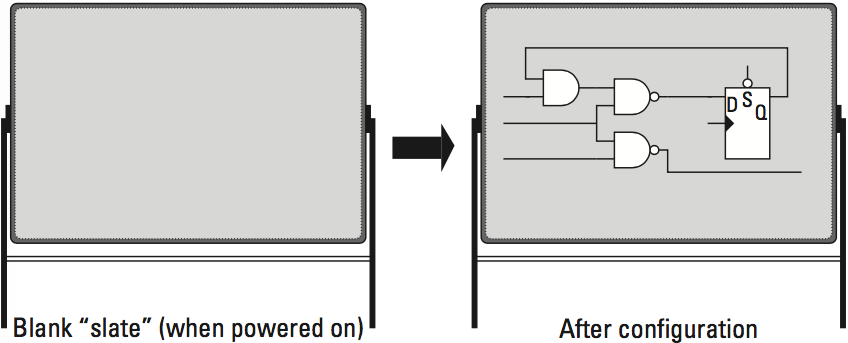
\includegraphics[width=0.75\textwidth]{img/rt-board.png}
      %   \caption{Ilustração em alto nível do funcionamento interno do FPGA. Fonte: \cite{Sass2010}.}
      %   \label{fig:rt-board}
      %\end{figure}

      %A seguir, será descrito a tecnologia que consiste os \hardwares\ reconfiguráveis, em especial o FPGA, e as respectivas linguagens de descrição de \hardware.

   %\subsection{Sua Tecnologia}
      % PLD
      %Para introduzir alguns conceitos, é importante destacar o que são os dispositivos lógicos programáveis (PLDs, do inglês \textit{Programable Logic Devices}).
      %Às vezes chamados de dispositivos lógico programáveis em campo (FPLD, do inglês \textit{Field-Programmable Logic Device}), podem ser adaptados para criar muitos dispositivos digitais, desde simples portas lógicas até estruturas complexas.
      %\cite{tocci2003sistemas, Plessl2003} dizem que com um investimento de capital pequeno, qualquer empresa pode comprar os \softwares\ de desenvolvimento e \hardware\ necessário para programar PLDs para seus projetos digitais.
      %De modo geral, os PLDs são descritos como pertencendo a três tipo diferentes sendo eles os dispositivos lógicos programáveis simples (SPLD), dispositivos lógicos programáveis complexos (CPLDs, do inglês \textit{Complex Programmable Logic Devices}) e arranjo de portas programáveis em campo (FPGA) sendo o último tipo abordado neste trabalho \cite{Brown1996}.

      %LUTS
      O FPGA, segundo \cite{tocci2003sistemas}, constitui-se de vários módulos lógicos pequenos, independentes, programáveis e interconectados para criar funções maiores.
      É composto principalmente \ffs\ e de \luts,\ que podem ser de dois tipos \luts\ e \luts RAM.
      
      De acordo com a quantidade de recursos disponíveis por meio do FPGA é possível implementar inúmeros projetos digitais, como por exemplo, funções de processamento de imagem, algoritmos de redes de computadores, algoritmos criptográficos e \textit{soft}-processadores completos \cite{Plessl2003, Choi2016}.
      Uma das principais formas de sintetização é utilizando Sintetização em Alto Nível (HLS, \textit{High Level Synthesis}).
      
      %
      %Uma arquitetura geral simplista de FPGA é exibido na Figura~\ref{fig:rb-arch_fpga}.
      %Nela os quadrados menores situado nas laterais são blocos de I/O que podem ser configurados para fornecer recursos de entrada, saída ou bidirecionais.
      %Os quadrados maiores situados no interior são as LUTs, usados para guardar dados que entram ou saem e realizar as operações lógicas.
      %Os canais que interligam os blocos entre si são estabelecidas por meio de conexões que passam pelas linhas e colunas nos canais entre esses blocos e possuem a funcionalidade de serem interconexões programáveis \cite{tocci2003sistemas}.
      %A tecnologia interna de um FPGA consiste basicamente de um arranjo de blocos lógicos, canais de roteamento para interconexão de blocos lógicos e blocos de entrada e saída de sinais em torno do circuito.
      %FPGAs baseado em SRAM (do inglês \textit{Static Random Access Memory}) utilizam células SRAM para controlar a funcionalidade de blocos lógicos e entrada e saída de sinais bem como as rotas, e pode ser reprogramado arbitrariamente em nível de circuito, muitas vezes, baixando um novo \textit{stream} de dados de configuração para o dispositivo.
      %Possuem milhões de portas de lógicas programáveis, bilhões de transistores, além de outros blocos de \hardware\ dedicados como memórias embarcadas e multiplicadores de ponto-fixo tornando-os um dos circuitos integrados (CI) mais densos existente \cite{Choi2016}.

      % tecnologia e energia
      %Segundo \cite{tocci2003sistemas},
      %tais maravilhas de flexibilidade de projetos digital podem fornecer uma série de opções de projeto sendo voltados para indústria e até mesmo educação.
      %ao utilizar tecnologia CMOS, o consumo de energia do chip é relativamente baixo comparado com outras tecnologias, podendo ser confeccionado em nível de tensão elétrica, frequências e cargas para os sinais de I/O.
      %O mercado fornece diferentes graus de velocidade de FPGA a fim de que o projetista utilize o mais adequado ao projeto.
      %Entretanto, um dispositivo FPGA pode ser configurado para um número infinito de projetos e isso implica na não possibilidade de afirmar o montante de dissipação de energia para um dispositivo FPGA.
      %O \software\ Quartus II tem duas ferramentas para estimular o montante de uso de energia para uma aplicação.
      %O \textit{PowerPlay Early Power Estimator} é usado durante os estágios iniciais do projeto para estimar a magnitude de potência do dispositivo.
      %Dessa forma, FPGAs são chips que podem ser programados instantaneamente para funções de qualquer circuito digital \cite{Choi2016}.

      % Importancia
      %\cite{tocci2003sistemas, Plessl2003} citam ainda que o motivo de PLDs estarem dominando o mercado é o fato de que, como são dispositivos programáveis, a mesma funcionalidade pode ser obtida com um circuito integrado (CI) ao invés de diversos circuitos individuais.
      %Isso significa maior confiabilidade, menor espaço ocupado na placa, consumo de energia, complexidade de desenvolvimento e, geralmente, menor custo de fabricação.

      \begin{comment}
      \subsubsection{\textit{Hard} e \textit{Software Cores}}
         % Utilização de um processador sintético ou físico
         A unidade de processamento central (CPU, do inglês \textit{Central Processing Unit}) nesses tipos de sistema pode estar disposta em duas naturezas distintas, sendo estas \textit{hard} e \textit{soft} \cores.
         A primeira é um \core\ dedicado, ou seja, um pedaço de circuito integrado dentro (ou não) de um FPGA, enquanto a segunda é feita por meio da sintetização de um processador no FPGA utilizando seus recursos lógicos, ou seja, \design\ e sintetização na placa.
         Independente de sua natureza, o sistema, cujo nome torna-se SoC FPGA (do inglês, \textit{System-on-Chip} FPGA), terá a seguinte arquitetura exibida na Figura~\ref{fig:rb-soc}.
         
         \begin{figure}[h] 
            \centering
            \vspace{-1em}
            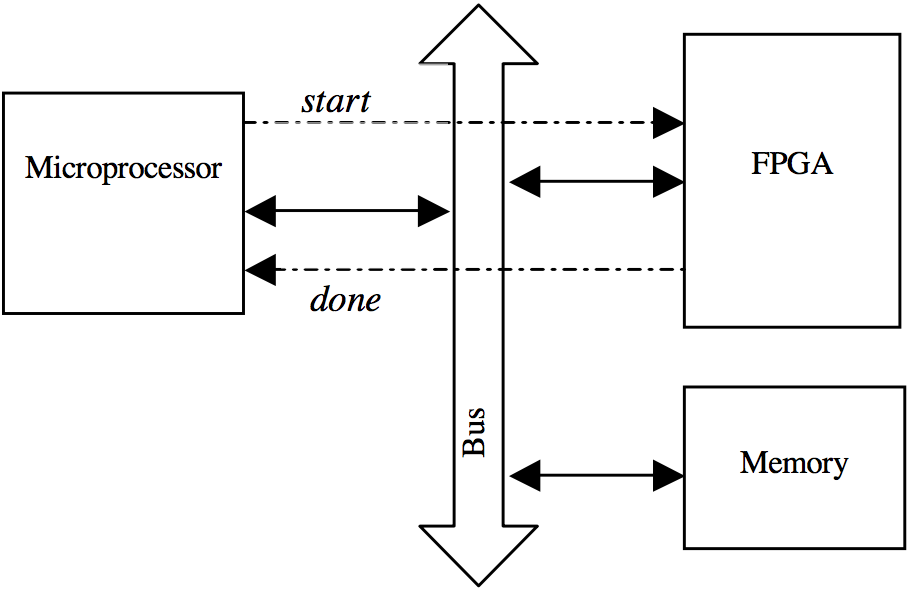
\includegraphics[width=0.35\textwidth]{img/into-soc.png}
            \caption{Visão geral de um SoC FPGA. As setas representam os barramentos de comunicação entre os principais componentes.}
            \label{fig:rb-soc}
         \end{figure}
         
         Cada um tipo de \core\ possui suas vantagens.
         Ao utilizar um \textit{hard} \core, é possível utilizar todos seus recursos obtendo máxima performance nas atividades executadas, a utilização de um \textit{soft} \core\ permite a extensão/configuração de sua arquitetura \cite{Plessl2003}.

         %Um das maiores barreiras para o \design\ de projetos em FPGA é a necessidade de uso de linguagens de descrição de \hardware.
         %Elas serão descritas a seguir.
      \end{commaent}
   \subsection{Profiling} \label{sec:profile}
         \Profile\ é uma procedimento para auxiliar o desenvolvedor a coletar informações do \software\ em tempo de execução.

         O processo é feito ao colocar o \software\ referencial (programa a ser analisado) como entrada representativa na ferramenta e a coleta é realizada em várias partes da aplicação ao longo de sua execução neste.
         Uma das técnicas do \profile\ de mensurar uma aplicação é na realização de interrupções periódica no programa e amostrar o seu \textit{program counter}.
         Dessa forma, é possível utilizar um histograma para contar quando um programa é interrompido em um endereço particular e a partir dessa informação, calcular a fração aproximada do tempo total de execução gasto em suas partes \cite{Graham1982}.
         %Distribuições GNU/Linux possuem a ferramenta \texttt{gprof} na qual avalia procedimentos enviados por parâmetro, realizando o cálculo de tais informações de \software\ \cite{Graham1982}.

        \end{comment}

%!TEX root = ../main.tex
% !TeX encoding = UTF-8
\subsection{Trabalhos Relacionados}  \label{chap:relacionados}
    % Embedded
    %O desenvolvimento com foco em SE ou microcontroladores já é pesquisado amplamente como os trabalhos de \cite{Ernst1993, Gupta1995, Hardt1995, Gajski1994, Bolsens1997}, publicados na década de 90.
    
    Em \cite{Mei2000} além do particionamento, os autores apresentam uma abordagem de escalonamento para SE dinamicamente reconfigurável (DRESs, do inglês \textit{dynamically reconfigurable embedded systems}). % no qual possuem como projeto um processador de propósito geral junto com um FPGA sendo este reconfigurável em tempo de execução para reduzir custos.
    Neste trabalho os autores fornecem análises dos tempos de configuração e reconfiguração parcial do FPGA e mostram que o algoritmo proposto resolve o problema de particionamento e escalonamento dos DRES.
    
    Em \cite{Arato2003} os autores descrevem algumas versões do problema de particionamento para sistemas de tempo real e custo restringido, provando que são problemas $ \mathcal{NP} $-difícil.
    Adicionalmente, apresentam uma abordagem com programação linear inteira, resolvendo o problema de forma otimizada, e uma abordagem utilizando algoritmo genético, na qual encontram-se soluções próximas ao ótimo global.
    
    O trabalho em \cite{Mann2007} descreve uma primeira tentativa para um algoritmo exato para o problema de particionamento.
    Utiliza um esquema no qual implementa-se a estratégia \textit{branch-and-bound} como um \textit{framework}.
    %Em sua implementação, realizaram várias investigações para incrementar a eficiência do algoritmo, incluindo várias técnicas sendo elas: \textit{lower bounds based on LP-relaxation}, uma mecânica de inferência customizada, condições não-triviais necessárias baseadas num algoritmo \textit{minimum-cut}, e diferentes heurísticas com passos pré-otimizados.
    %Este também pode ser generalizado a fim de incluir mais de uma restrição, permitindo o \designer\ prescrever quais itens devem estar em qual nível de projeto.
    Eles demonstram que problemas de particionamento altamente complexos podem ser resolvidos em tempo razoável.
    %Citam ao final que o resultado obtido é em entorno de dez minutos mais rápido que algoritmos exatos anteriores baseados em programação linear inteira para os testes realizados.
    
    Pesquisas mais recentes, como a de \cite{BenHajHassine2017} procuram aplicar otimizações sobre o tempo de execução e gasto energético para processadores baseados em produtos embarcados, por meio de particionamento.
    %Propõem alcançar um particionamento de grafos à procurar o melhor conjunto da relação energia e tempo de execução.
    Comparado com outras heurísticas, o algoritmo mostra-se ser mais adequado para aplicações que necessitam do equilíbrio no \textit{tradeoff}.
    
    Trabalhos como o de \cite{Trindade2016} utilizam algoritmos genéticos para solucionar o problema de particionamento em SE.
    Propõem novas abordagens usando técnicas de verificação baseadas nas teorias de módulo de satisfação (SMT, do inglês \textit{satisfiability modulo theories}).
    %Apresentam um exemplo de particionamento, modelam e solucionam-o usando três diferentes técnicas sendo a principal ideia é aplicar mo método de verificação SMT ao particionamento \hs, e por fim, comparar os resultados com técnicas de otimizações tradicionais como ILP e GA.
    
    
    %concluindo tudo que foi dito
    Os trabalhos citados buscam o estudo do desempenho e \design\ de SE no geral por meio de particionamento, mas nenhum com foco em \wearables.
    
    
    Em \cite{Jozwiak2017} os autores apresentam uma extensa revisão da literatura considerando vários aspectos de um SE, bem como suas tecnologias de \design,\ com foco em sistemas móveis modernos incluindo \wearables.
    %Cita-se dois paradigmas de desenvolvimento para SE sobre sistema multi-processados heterogêneos, sendo eles o de sistemas \textit{life-inspired} e sistemas \textit{quality-driven}.
   % O \textit{life-inspired} (inspirado pela vida) especifica princípios básicos, características e organizações funcionais e estruturais de um SEe por meio da analogia à vida de um organismo inteligente, além de soluções de mecanismos e arquiteturas de sistemas para implementar tais princípios.
    %Já o \textit{quality-driven} (orientado pela qualidade) é o \design\ de dispositivos que necessitam satisfazer as exigências de tempo real, baixo consumo de energia, entre outros e assim, especifica qual a nova qualidade do sistema a ser requerida e como esta meta é obtida.
    %De forma a facilitar a compreensão, \cite{Jozwiak2017} define qualidade de uma solução sistêmica proposto como o total de sua eficácia e eficiência na resolução do problema real.
    %Eficácia entende-se como o grau em que uma solução atinge seus objetivos e a eficiência o grau em que uma solução usa recursos para realizar seus objetivos e juntas determinam o grau de excelência.
    %Elas são expressas em termos de parâmetros mensuráveis, o que é necessário para implementar o design \textit{quality-driven}.
    %Entretanto, é descrito ao final que, enquanto \designers\ aprenderam bastante na construção de plataformas de \hardware\ heterogêneos altamente paralelos, os métodos e ferramentas automatizadas para a sua programação e o paralelismo do algoritmo, bem como o \codesign\ coerente da arquitetura \hs\ ainda são atrasados perante à tecnologia.
    % wearable fpga
    Além deste, é possível ver em \cite{Plessl2003, Ahola2007, Abdelhedi2016, Narumi2016, Lee2015} trabalhos que estudam \wearables\ junto de FPGA, mas nenhum deles utilizam a técnica de particionamento como meio para seu \design.
    
    % conclusao
    Este trabalho portanto consiste na análise do problema de particionamento \hs,\ com foco em \design\ de sistemas \wearables\ em plataforma FPGA.


%!TEX root = ../main.tex
% !TeX encoding = UTF-8
\section{Princípios do Particionamento de Sistemas Gerais} \label{chap:design}
    
    A seguir serão descritos tópicos utilizados para o entendimento do particionamento, seguindo conceitos estabelecidos por vários trabalhos como \cite{Arato2003, Arato2005, Mann2007, BenHajHassine2017, Sass2010}.
    Esses tópicos são necessários para o entendimento básico dos arcabouços metodológicos de \codesign\ e o seu particionamento para sistemas, em especial para \wearables, além de definições formais sobre.
    
    %Os tópicos a seguir são a Definição de \Design\ de Referência de \Software\ (Seção~\ref{sec:GCF}) bem como o Ganho de Performance (Seção~\ref{sec:ganho_performance}) em tais sistemas, o Particionamento \HS\ para Sistemas \Wearables\  (Seção~\ref{sec:desenvolvimento}) e a Proposta de Procedimento Analítico (Seção~\ref{sec:proposta}).
    
    %\subsection{Fundamentação Matemática} \label{sec:GCF}
    
    É possível descrever sistemas livre de especificações formais por meio de descrições de protótipos simples, conhecidos como \Design\ de Referência de \Software\ (DRS)\cite{Sass2010}.
    %Com ele, é possível ter uma generalização de uma especificação sistêmica, eliminando quaisquer tipo de incertezas sobre o comportamento do sistema ao realizar uma análise sobre, sendo este podendo ser representado por diversas formas.
    % além de outras como o fato de que sua especificação pode ser analisada por ferramentas computacionais, e gerando modelos aut.
    %
    %Assumindo que o \design\ de referência de \textit{software} já exista,
    %Primeiramente, será demonstrado matematicamente como computação está em \design\ referencial de \sof%htware\ para que depois, isso possa nos auxiliar na decisão do que deverá ser implementado em nível de \hs.
    Dessa forma, o algoritmo a ser analisado também pode ser representado como grafo de rotinas, chamado de Grafo de Controle de Fluxo (GCF) \cite{Mann2007}.
    Ele é definido por $C = (B, F) \label{eq:subrotina}$
    %\begin{equation}
    %   C = (B, F) \label{eq:subrotina}
    %\end{equation}
    onde $B$ são vértices que representam as tarefas %\footnote{De modo geral é um trecho de código sequencial maximal, onde só existe um ponto de entrada e um ponto de saída.}
    %http://www.dcc.ufrj.br/~gabriel/microarq/Escalonamento.pdf
    e $ F $ são arestas que indicam todas as possibilidades de caminhos entre elas.
    
    \begin{comment} %figura
    Utilizando o exemplo da Figura \ref{fig:blocos_basicos}, o primeiro grupo \A\ é um bloco não básico porque não é maximal, ou seja, a primeira instrução \texttt{store word with update} deveria estar incluída ao grupo para conter o número máximo de instruções possuindo apenas um ponto de entrada e saída.
    Grupo \B\ é um bloco básico e o grupo \C\ não se define como bloco básico pois existe duas entradas para o bloco, sendo elas na instrução \texttt{store word} e também pelo \texttt{branching} direcionado para \texttt{L2}.
    
    Dessa forma, fazendo uma relação entre o processo de gerar um Grafo de Controle de Fluxo a partir de um código em alto nível, a Figura~\ref{fig:f3-6} exibe um pequeno código demonstrativo na qual o processo ocorrerá.
    A partir do código em alto nível (Figura~\ref{fig:f3-6} \textit{a)}) é identificado os blocos básicos de acordo com o compilador\footnote{Deve-se atentar que, só é possível identificar blocos básicos em um arquivo em linguagem de programação \textit{C} desde que se saiba qual compilador foi utilizado para emitir o código \assembly.} utilizado.
    Neste exemplo, utilizou-se de um compilador para \texttt{PowerPC}\footnote{Arquitetura que utiliza RISC como arquitetura do conjunto de instruções.} onde os blocos básicos são identificados pela Figura~\ref{fig:f3-6} \textit{b)}.
    Por fim o GCF resultante deste processo, representado pela Figura~\ref{fig:f3-6} \textit{c)}.
    
    \begin{figure}[!ht] \centering
    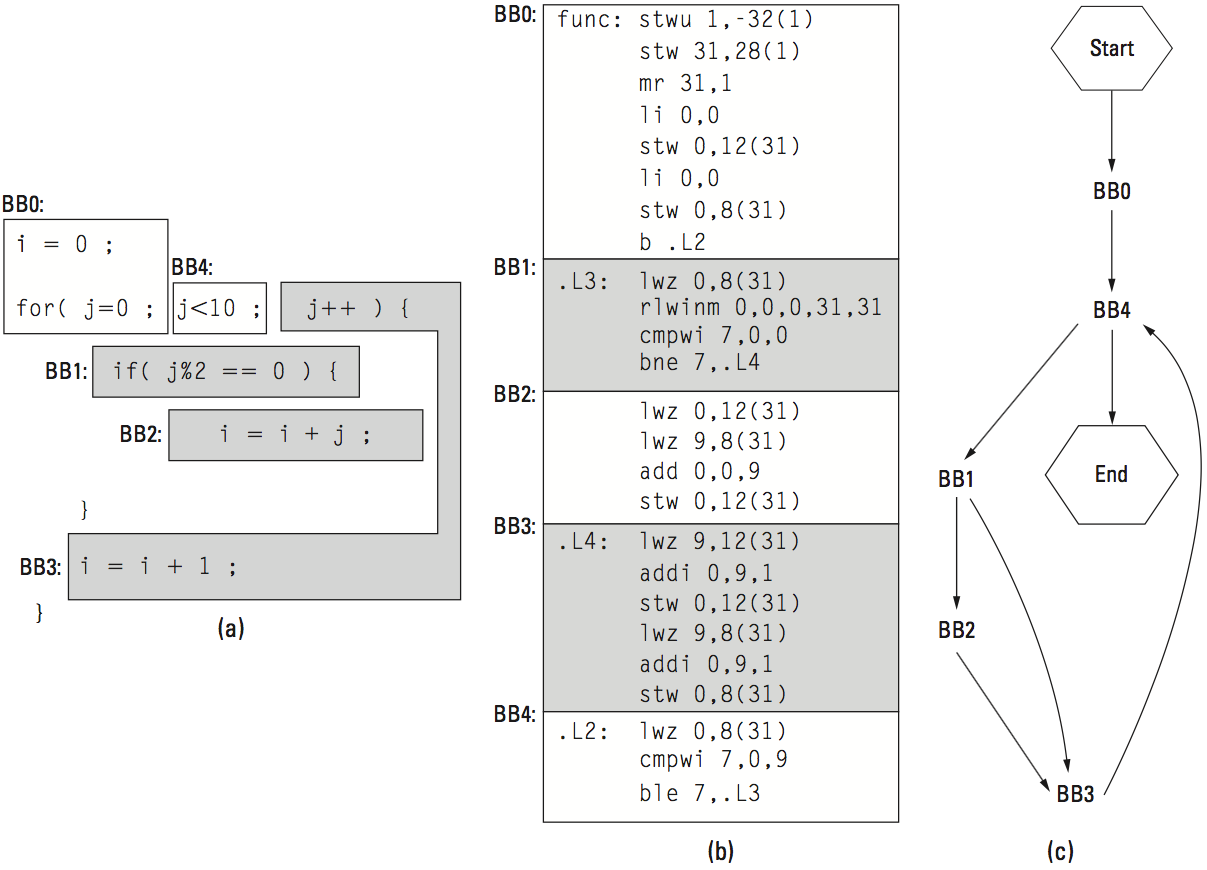
\includegraphics[width=0.35\textwidth]{img/f3-6.png}
    \caption{Identificação de blocos básicos e a representação por meio de um grafo não atrelado à uma especificação \hs.}
    \label{fig:f3-6}
    \end{figure}
    \end{comment}
    
    A decomposição de um DRS pode gerar dois componentes: uma porção a ser realizada em \hardware\ e outra executada em \software.
    Essa decisão de divisão é chamada de Problema de Particionamento.
    %Segundo \cite{Sass2010}, para sistemas em FPGA, o particionamento é um sub-problema de um problema mais geral no âmbito de \codesign, onde refere-se ao \design\ cooperativo entre engenheiros de \hs\ para um desenvolvimento mais eficiente.% envolvendo \textit{stakeholders}, por exemplo.
    %Para continuar, deve-se definir alguns conceitos básicos, descritos na Seção \ref{sec:gc}.
    
    \subsection{Definição Formal do Problema de Particionamento \HS} \label{sec:gc}
        %Modelado uma sub-rotina de um DRS utilizando o GCF, definido na Seção \ref{sec:GCF}, agora será descrito uma nova notação, chamada de Grafo de Chamada (GC) utilizado para o entendimento da partição.
        Um Grafo de Chamada (GC) consiste num conjunto de GCFs, um por sub-rotinas, ou seja, $\mathcal{C} = {C_0, C_1, \dots C_{n-1}}$
        %
        %\begin{equation}
        %   \mathcal{C} = {C_0, C_1, \dots C_{n-1}}
        %\end{equation}
        %
        %onde $ C_i = (V_i, E_i) $
        onde $ C_i = (B_i, F_i) $ representa o GCF de uma sub-rotina $ i $. %, como mostrado na Equação~\ref{eq:subrotina}.
        Sendo assim, o grafo estático de chamada da aplicação completa é escrito por $\mathcal{A} = (\mathcal{C}, \mathcal{L}) \label{eq:a}$
        %
        %\begin{equation}
        %   \mathcal{A} = (\mathcal{C}, \mathcal{L}) \label{eq:a}
        %\end{equation}
        %
        onde \A\ representa uma aplicação específica e $ \mathcal{L} \subseteq \mathcal{C} \times \mathcal{C} $ é um subconjunto do plano cartesiano\footnote{Duas sub-rotinas são relacionadas se podem ser determinadas que, no tempo de compilação, a sub-rotina $ i $ tem potencial de invocar a sub-rotina $ j $, ou seja, $ (C_i, C_j) \in \mathcal{L} $.} dos GCFs.
        
        %É assumido que os blocos básicos de cada sub-rotina são disjuntos, ou seja, cada bloco básico em uma aplicação pertence a exatamente um GCF.
        %Além do mais, é assumido também que um nó raiz para o GC é implícito, ou seja, uma sub-rotina é designada a iniciar a execução.
        %Nem todos os executáveis podem ser expressados nesse modelo.
        %Por exemplo, o manuseio de sinais e interrupções não são representadas e assim, não é possível determinar todos vértices $ F_i $ em uma dada sub-rotina $ C_i $ de um GCF antes da execução.
        %Uma outra forma é com o paradigma de orientação à objeto.
        %Ele depende do tempo de execução para conectar os métodos virtuais invocados e dessa forma, por \design, esse paradigma nos previne de saber todos os vértices antes da execução.
        %Para agora, será considerado que o modelo é suficiente para ser expressado em \design\ referencial de \software.
        
        %Um equívoco comum é de que uma definição formal de particionamento só aplica à separação de aplicação componentes de \hs, ou seja, a partição contém exatamente dois conjuntos.
        %Todavia, para fazer o problema mais tratável, é comum agrupar primeiramente operandos em recursos, ou seja, uma partição com um grande número de subconjuntos, e então mapeia esses recursos tanto em \hardware\ quanto \software.
        %Assumindo que esses recursos atuam razoavelmente bem \textit{clustered}, então a decomposição de uma aplicação em componentes de \hs\ pode ser dirigida por comparações de ganho de performance desse recurso contra outro situado no outro conjunto.
        
        %Definidos os conceitos prévios, será definido agora, formalmente, o conceito de uma partição.
        
        Com esses conceitos definidos, é possível definir-se também uma partição como $ \mathcal{S} = \{S_0, S_1, \dots S_i\} $ sendo $ i $ quantidade de partições, e $U$ como o conjunto de todas as sub-rotinas.
        Assim, uma partição \Ss\ de um conjunto universal $ U $ é definida como um conjunto de subconjuntos de $ U $, podendo ser definida como
        %
        \begin{eqnarray}
        \bigcup_{S \in \mathcal{S}} S &=& U           \label{eq:part_form_1} \\
        \forall S, S' \in \mathcal{S} | S \cap S' &=& \emptyset  \label{eq:part_form_2}\\
        \forall S \in \mathcal{S}\ |\ S &\neq& \emptyset  \label{eq:part_form_3}
        \end{eqnarray}
        %
        onde a Equação~\ref{eq:part_form_1} diz que cada elemento de $ U $ é um membro de pelo menos um subconjunto $ S \in \mathcal{S} $, e as Equações~\ref{eq:part_form_2} e \ref{eq:part_form_3} dizem que os subconjuntos $ S \in \mathcal{S} $ são emparelhados, disjuntos e não vazios.
        Em outras palavras, cada elemento do nosso universo $ U $ termina exatamente em um dos subconjuntos de $\mathcal{S}$ e nenhum dos subconjuntos são vazios.
        
        Com isso, é possível aplicar o formalismo à $ \mathcal{A} $, se assumirmos que nosso universo é o conjunto de todas as tarefas $B$ de um dispositivo \wearable\ e, assim, $U$ são as partições de sub-rotinas
        %
        \begin{equation}
        U = \bigcup_{C \in \mathcal{C}} B(C) \label{eq:bigcup}
        \end{equation}
        %
        sendo esta a partição natural da aplicação, onde
        %
        \begin{equation} \small
        \mathcal{S}  = \left \{
        \underbrace{\left \{ b_0, b_1, \dots b_{i-1} \right \}}_{\textnormal{sub-rotina }C_0},
        \underbrace{\left \{ b_i, b_{i+1}, \dots \right \}}_{\textnormal{sub-rotina }C_1},\dots
        \underbrace{\left \{ b_j, b_{j+1}, \dots \right \}}_{\textnormal{sub-rotina }C_{n-1}}
        \right \}
        \end{equation}
        
        
        \makeatletter
        \def\@eqnnum{{\normalsize \normalcolor (\theequation)}}
        \makeatother
        
        %
        O propósito é a reorganização de $U$ em um particionamento com dois subconjuntos  $ \mathcal{S} = \{S_0, S_1\} $, sendo eles \hs.
        Dessa forma, teremos uma nova partição \Ss$'$ gerando um novo resultado $ \mathcal{A}’ = (\mathcal{C}’, \mathcal{L}’) $, inferido a partir da reorganização da partição $ \mathcal{S} $.
        
        O segundo passo é mapear cada subconjunto de $ \mathcal{S}' $ para ambos \hs,\ como é exibido na Equação \ref{eq:part_final}.
        
        { \small
        \begin{equation}
        \mathcal{S}'\!=\!\left \{
        \underbrace{
        \underbrace{
        \left \{ b_0, b_1, ... b_{i-1} \right \}
        }_{\textnormal{sub-rotina }C_0},
        ...
        \underbrace{
        \left \{ b_j, b_{j+1}, ... \right \}
        }_{\textnormal{sub-rotina }C_{n-i}}
        ...
        }_{\textnormal{\software}};
        \ 
        \underbrace{
        \underbrace{
        \left \{ b_i, b_{i+1}, ... \right \}
        }_{\textnormal{sub-rotina }C_{n-1}}
        ...
        }_{\textnormal{\hardware}}
        \right \} \label{eq:part_final}
        \end{equation}
        }
        
        %A seguir será explicado como o desempenho pode ser utilizada para guiar o particionamento.
        %Para explicar como performance pode ser utilizada para guiar o particionamento, será descrita uma métrica simples chamada taxa de execução\footnote{Taxa de execução é a velocidade na qual um sistema computacional completa uma aplicação, e em um sistema de plataforma FPGA olhamos também para o \hardware\ para melhorar sua taxa de execução.} a seguir.
    
    
    \subsection{Desempenho como Guia ao Particionamento \HS} \label{sec:ganho_performance}
        \subsubsection{Ganho de Desempenho}
            %É parcialmente motivada pelo fato de que: \textit{a)} o ganho de desempenho é relativamente fácil de ser mensurado e \textit{b)} por causa de que, de todas as métricas comumente utilizadas, \speedup\ é frequentemente a mais importante.
            Para aplicações em geral pode estar no acúmulo de pequenos ganhos.
            Entretanto, diferente de algoritmos em \software\ no qual tem-se análise de ordem de complexidade, em \hardware\ não possui-se um guia geral para comparação.
            
            
            % tempo mudanca de estado, configuracao, latencia
            \begin{comment}
            Por fim, a `interfaceação' entre \hs\ requer tempo e este custo também precisa ser contabilizado.
            Pode-se aproximar deste custo pela aproximação do montante total do estado que necessita ser transferido ou o custo de configuração e latência.
            Em ambos os caso, são representados por $ m $ para recursos $ i \in \mathcal{H} $, sendo $\mathcal{H}$ o conjunto de recursos do \hardware.
            \end{comment}
            % y é speedup
            O ganho, ao comparar uma solução \hs\ contra uma solução puramente \software,\ é tipicamente mensurado por meio do \speedup, e pode ser obtido utilizando a Equação~\ref{eq:speedup1}.
            Utiliza-se $ \gamma $ para sua representação, permitindo comparar recursos diferentes para determinar melhores particionamentos.
            %Qualquer subconjunto de tarefas que não produzem um maior ganho de desempenho, podem ser desconsiderados, ou seja, somente $ \gamma > 1.0 $ são considerados recursos candidatos.
            %Então quando considerado se um conjunto particular de blocos básicos deveriam ser mapeados ao \hardware\ ou \software, estamos interessados em seu ganho em \speedup, ou seja
            %
            \begin{equation}
            \gamma =
            \frac{
            \textnormal{\textit{hardware speed}}
            }{
            \textnormal{\textit{software speed}}
            }
            =
            \frac{
            \frac{
            1
            } {
            \textnormal{\textit{hardware time}}
            }
            } {
            \frac{
            1
            }{
            \textnormal{\textit{software time}}
            }
            }
            =
            \frac{
            \textnormal{\textit{software time}}
            } {
            \textnormal{\textit{hardware time}}
            } \label{eq:speedup1}
            \end{equation}
            %
            Mais especificamente, interessa-se no ganho de desempenho individual de cada recurso o que pode ser definido como $ \gamma(i), i \in \mathcal{C}\ |\ \gamma(i) =\ ^s\!/_h $.
            Para que um algoritmo em \hardware\ seja mais performático, deseja-se que $\gamma > 1$.
            %
            %onde $ h(i) $ e $ s(i) $ são o tempo de execução de uma implementação de um recurso $ i $ em \hs\ e a função $ m(i) $ é o tempo que se leva para sincronização, ou seja, o tempo que leva para guiar um dado entre o processador e o item reconfigurável.
            \begin{comment}
            %Assumindo por um momento que usaremos esse recurso separado em nosso \design, deve-se questionar sobre o quão rápido é a aplicação.
            A velocidade da aplicação é dependente dos ganhos de desempenho do recurso e o quão frequentemente ele é utilizado no DRS.
            Pode-se ter essa fração do tempo gerado de um recurso particular $ p(i) $ a partir de informações de \textit{profile} e dessa forma o \speedup\ da aplicação no geral será
            %
            \begin{equation}
            \Gamma = \left [
            (1 - p(i))
            +
            \frac{
            p(i)
            }{
            \gamma(i)
            } \right ]^{-1}
            \end{equation}
            %
            A inversão representa que estamos movendo entre taxa de execução e tempo de execução para manter o sentido de ganho de desempenho.
            
            %A partir dessa equação, podemos observar que aumentando a velocidade do \hardware\ de um único recurso tem-se menos e menos impacto no desempenho da aplicação a medida que sua frequência decresce.
            
            %Para aumentar o desempenho sistêmica de uma aplicação no geral, também deve-se aumentar o sistema com múltiplos recursos que aumentará o desempenho de componentes individualmente assim como aumentando a fração agregada de tempo gasto em \hardware.
            Para computar o \speedup\ de múltiplos recursos em \hardware, deve-se avaliar o ganho sistêmico de um conjunto de recursos $ \mathbb{D} $.
            %Para estimar o desempenho desta partição, podemos adicionar recursos e rearranjar os termos para ter um ganho de desempenho almejado no geral,
            Assim, para o cálculo de desempenho dos recursos, utiliza-se da Equação \ref{eq:d_final}.
            %
            \begin{equation}
            \Gamma (\mathbb{D}) =
            \left [
            \sum _{i \in \mathbb{D}} \left (
            \frac{
            p(i)
            }{
            \gamma(i)
            }-p(i)
            \right) + 1
            \right ]^{-1} \label{eq:d_final}
            \end{equation}
            \end{comment}
        
        
        
        \subsubsection{Recursos Finitos em Componentes Eletrônicos} \label{sec:recursos}
            %Uma hipótese de consideração de recursos seria implementar tudo em nível de \hardware\ para maximizar o desempenho, o que no caso, ignoraria todos os custos de desenvolvimento e recursos finitos.
            %Uma plataforma FPGA possui um número finito de recursos disponíveis destes e, com essa estratégia, a maioria das aplicações reais iriam exceder esse limite disponível.
            
            %Uma plataforma FPGA possui um número finito de recursos disponíveis.
            %Dessa forma, realizou-se a contagem do número de recursos em \hardware\ requeridos para cada algoritmo candidato particionado.
            Um FPGA terá um valor escalar total $ r_{FPGA} $, que representa o total de números de \luts\ disponíveis para sintetização.
            Então $ r(i) $ pode ser usado para representar a quantidade de recursos requerida por cada algoritmo $ i $.
            Fazendo uma simples relação, tem-se que $ \sum_{i \in \mathbb{D}} r(i) < r_{FPGA} $ restringe quão largo $ \mathbb{D} $ pode crescer, onde $ \mathbb{D} $ é o conjunto de algoritmos candidatos.
            
            Uma típica plataforma FPGA moderna tem múltiplos tipos de recursos além de \luts,\ como memória, blocos DSP, etc., sendo a quantidade de recursos de cada tecnologia representados matematicamente por  $r_{Logic\ Cells}$, $r_{Memory}$, $r_{DSP}$, $r_{n-1} $, respectivamente.
            Dessa forma, podem ser representados por um vetor de recursos
            %
            $ \vec{r}_{FPGA} = (r_{Logic\ Cells}, r_{Memory}, r_{DSP}, \dots r_{n-1} ) $
            %
            %
            %         \begin{equation} \footnotesize 
            %            \vec{r}_{FPGA} =
            %            \begin{pmatrix}
            %            r_{Logic\ Cells} \\
            %            r_{Memory}\\
            %            r_{DSP}\\
            %            \vdots \\
            %            r_{n-1}
            %            \end{pmatrix}
            %         \end{equation}
            %
            e com isso,
            %
            %\begin{equation}
            $\sum_{i \in \mathbb{D}} \vec{r}(i) < \vec{r}_{FPGA}$.
            %\end{equation}
            %
    
    
    \subsection{Avaliação do Wearable}
        %\todo[inline]{ explicando como a teoria da secao III se aplica na pratica ao seu experimento.} 
        
        Enquanto o desempenho do \wearable\ é avaliada pelo tempo de execução do sistema segundo a Equação~\ref{eq:speedup1}, a alocação de recursos deve ser analisada, tanto em cada um dos \hardwares\ dos algoritmos gerados por HLS, quanto para o sistema como um todo, respeitando o limite de recursos $ \vec{r}_{FPGA}$.
        
        Dessa forma, será utilizado \A$_{i}$\ para descrever separadamente as implementações dos $i$ códigos candidatos e \Ss$_{j}$\ referencia-se às implementações dos $j$ sistemas sintetizados.
        %
        Com a diferenciação entre \A$_{i}$\ e \Ss$_{j}$\ (parte e todo do sistema)\ é possível analisar tanto as implementações dos módulos gerados por HLS separadamente, quanto os sistemas finais na alocação de recursos.
        
        
        
        %vou garar cada algoritmo
        %e vou analisar cada algoritmo
        
        %Depois vou adicioanr ao seus sistemas
        % e analizar o quanto cada sistema ficou com os hardware novos
        
        
        %\todo[inline]{a}
        
        
        %O particionamento será aplicado à determinados códigos pertencentes ao \wearable,\ nomeados como \A$_{i}$. %,\ e realizando análises executando-os em nível de \software\ via código e em \hardware\ via HLS.
        %Com a geração dos códigos em \hardware\ utilizando HLS, é possível contabilizar os gastos referentes a cada módulo \A$_{i}$\ separadamente.
        
        %Além de cada módulo \A$_{i}$,\ ao construir o sistema que compõe o \wearable\ como um todo definido como \Ss$_{i}$, também será possível quantificar os seus gastos.
        
        
        %Além da análise de desempenho provinda pelo particionamento, será possível conferir se o sistema \Ss$_{i}$\ junto de seu particionamento \A$_{i}$\ aplica à restrição de ser menor que $ \vec{r}_{FPGA}$
        
        
        %Com a junção do sistema e o algoritmo é possível ver se $ < \vec{r}_{FPGA}$.
        
        %Assim, para referenciar somente os códigos candidatos ao longo desde documento utilizou-se de \A$_{i}$\ e para os códigos que estão juntos de seus sistemas de processamento e sua interface de comunicação utilizou-se de \Ss$_{i}$, ficando mais claro quando mencionar sobre a parte ou o todo do sistema.

%%!TEX root = ../main.tex
% !TeX encoding = UTF-8
%\chapter{O Particionamento de \HS\ para Sistemas \Wearables} \label{chap:desenvolvimento}
   \section{O Particionamento de Hardware e Software para Sistemas Wearables} \label{sec:desenvolvimento}

      %De início, será considerado como aplicaçãåo \wearable\ um conjunto de instruções organizadas, e como visto na Seção \ref{sec:gc}, esta também representada por uma coleção de grafos de controle de fluxo, ou seja, GC, especificando a sua ordem de execução.
      A partir deste, será feito análises a fim da procura de um particionamento que atenda aos requisitos de dispositivos \wearables\ como poder de processamento sem o \textit{trade-off} de energia, além de miniaturização, confiabilidade e outros.

      %Após esclarecidos algumas definições prévias (Seção~\ref{sec:definicoes_previas}), será apresentado o problema na Seção~\ref{sec:declaracao_problema}.
      %Alguns fatores podem ajudar nas decisões de particionamento tal como expectativa de ganho de performance (Seção \ref{sec:ganho_performance}) e os recursos utilizados em \hardware\ (Seção \ref{sec:recursos}).%, a forma na qual são usados e, talvez os mais importantes, quanto de sobrecarga de comunicação a decomposição impõe (Seção \ref{sec:comunicacao}) \todo{deixar?}e dificuldade de implementar um conjunto específico em \hardware\ (Seção \ref{sec:dificuldades}).\todo{organizar}


   \subsection{Declaração do Problema} \label{sec:declaracao_problema}
      %Nesta seção serão apresentadas as declarações matemáticas do problema de agrupamento de instruções em recursos e seus mapeamentos em \hardware\ ou \software, ou seja, o particionamento \hs.
      %Segundo \cite{Sass2010}, a forma mais comum de transcrever é descrever manualmente o \core\ com um HDL utilizando \design\ referencial de \software\ como especificação, método utilizado para descrever o problema.

      No particionamento, muitos problemas práticos impactam diretamente na performance do sistema.
      Nem todos os problemas podem ser incorporados num modelo analítico \cite{Wang2016}, e por isso, só podemos esperar que as soluções matemáticas produzam uma resposta aproximada ao problema de particionamento ao utilizar a declaração formal, pois muitas das entradas do modelo são estimadas ou aproximações no qual futuramente degrada a fidelidade de resultados.
      %%Este é um fato relevante pois com isso, resolvendo o problema de particionamento `no papel', tem-se um particionamento que é próximo ao ótimo.
      %%Assim, cabe ao \designer\ ser habilidoso em usar os guias e projetar uma solução mais refinada.
      Dessa forma, é mais eficiente usar uma combinação de técnicas \textit{ad hoc} e matemáticas para encontrar uma solução ótima ou aproximada como será feito, do que simplesmente confiar numa intuição.


      %\begin{comment}
      %\subsection{Declaração do Problema}
      %Já descrito as ferramentas matemáticas necessárias para descrever o problema fundamental do particionamento no Capítulo \ref{chap:revisao_bibliografica}, pode-se então descrever formalmente o problema em termos de variáveis. % e descrever um algoritmo \todo{algorit?}para encontrar uma solução aproximada.
      %
      %A ideia básica consiste em encontrar um particionamento para todos os blocos básicos de uma aplicação e então separá-los em \hs.
      Formalmente, procura-se por uma partição $ \mathcal{P} $ de todas as tarefas $ U $ de uma aplicação.
      %
      %$$ U = \bigcup_{C \in \mathcal{C}} B(C) $$
      %
      %$ C = (B,F) $
      Definida a partição e o universo, tem-se então um subconjunto $ \mathbb{C}\ |\ \mathbb{C} \subseteq U $, onde $ C \in \mathcal{C} $ é um vértice de um $ \mathcal{A} = (\mathcal{C}, \mathcal{L}) $.
      O conjunto $ \mathbb{C} $, chamado conjunto de candidatos, contém todos os recursos arquiteturais potenciais, ou seja, o subconjunto de $ U $ que é esperado para melhorar a performance do sistema se implementado em um \hardware\ reconfigurável.
      Devido ao limite de recursos, deve-se refinar para o subconjunto $ \mathbb{D} \subseteq \mathbb{C} $ que maximiza nosso métrica de performance.
      Assim, tem-se
      \begin{equation}
         \begin{array}{rrcl}
         \textnormal{max}                 & \Gamma ( \mathbb{D})               & ~   & ~                \\
         subject\ to & \sum_{i \in \mathbb{D}} \vec{r}(i) & < & \vec{r}_{FPGA}
         \end{array}
         \label{eq:constraints}
      \end{equation}
      %
      %Descrevendo isso algoritmicamente, uma abordagem seria encontrar todas as partições de $ U $, sintetizando e \textit{profiling} cada partição, e então, quantitativamente avaliar cada $ \Gamma $.
      %Entretanto, este é um problema linear inteiro devido à natureza de alocação e utilização dos recurso físicos do FPGA. %(Seção \ref{sec:pli})

      A seguir, será descrito como é feito uma abordagem para tal, seguindo estudos de \cite{Arato2003, Wang2016}.


   %\subsection{Metodologia Proposta}
   \subsection{Proposta do Procedimento Analítico} \label{sec:proposta}

      Neste, apresenta-se o algoritmo (Algoritmo \ref{alg:proposta}) e sua descrição classificadas por cada fim a ser alcançado.
      %Neste, será formulada uma proposta de metodologia analítica baseada nos conceitos propostos pela literatura, com o foco em componentes procedurais integrados à sistemas \wearables.
      %E com isso, o trabalho consiste em desenvolver seus respectivos grafos e realizar o particionamento a fim de encontrar uma solução aproximada, respeitando os seus requisitos de funcionamento.
      %
      %Tal metodologia, apresentada pelo Algoritmo~\ref{alg:proposta}, será considerada apenas como uma orientação para os passos a serem realizados, sendo então, uma proposta representativa do processo a ser realizado para a análise e decisão de particionamento.

      \begin{algorithm}[b] \footnotesize
         \SetKwData{itt}{it}
         \SetKwData{pl}{partition\_list}
         \SetKwData{complexSet}{how\_complex\_set\_is}
         \SetKwData{md}{matriz\_dados}
         \SetKwData{complexSet}{how\_complex\_set\_is}
         \SetKwFunction{graph}{make\_graph}
         \SetKwFunction{porte}{analyse\_complex\_set}
         \SetKwFunction{synth}{synthesize}
         \SetKwFunction{resources}{resources\_used}
         \SetKwFunction{die}{die\_used}
         \SetKwFunction{energy}{energy\_spent}
         \SetKwFunction{profiling}{profile}
         \SetKwFunction{performance}{performance\_analysis}
         \SetKwFunction{factor}{complexity\_factor}
         \SetKwFunction{ilp}{integer\_linear\_solve}
         \SetKwFunction{heuristic}{heuristic}
         \KwIn{a project description.}
         \KwOut{a partition solved.}

         %\BlankLine
         \Begin{

            \BlankLine
            \func{profiling}();
            \BlankLine

            %\tcp{extration project analyses}
            %\graph{Flow Control Graph}\;
            %\graph{Call Graph}\;
            %\complexSet $\leftarrow$ \porte{}\tcp*{verify if it is a big project}

            \BlankLine

            \If{exist partitions that can be synthesized}{
               \ForEach{partition project:\vars{it} $\in$ \vars{partition\_list}}{
                  \func{synth}(\vars{it});
                  \BlankLine
                  \func{resources}(\vars{it})\tcp*{analysis after synth}
                  \func{die}(\vars{it})\;
                  \func{energy}(\vars{it});
                  %\BlankLine


                  \func{performance}(\vars{it});
               }
               \BlankLine

               %\uIf(\tcp*[f]{verify if it is a small project}){\factor{\complexSet}}{
                  \func{ilp}(\vars{partition\_list})\tcp*{analyse quantitatively each $ \Gamma $}
               %}
               %\lElse{
                  %\heuristic{\vars{partition\_list})\;
               %}
            }
         }
         \caption{Metodologia de avaliação de \wearables.}
         \label{alg:proposta}
      \end{algorithm}
        \todo[inline]{atualizar algo e texto}
        \todo[inline]{melhorar}
      %Apresentado o procedimento metodológico, a seguir será listada cada função pertencente à metodologia acima, descrevendo suas funções e seu propósito no trabalho para a obtenção dos objetivos.
      %Para um maior compreendimento, serão divididos em quatro seções, sendo elas: visualização do projeto, síntese, análise de síntese, particionamento.

      \begin{enumerate}
         \item Procedimentos para visualização geral do projeto.
         %Por meio dos dados do \profile\ e a construção dos grafos, é possível ter uma visão geral, verificando se o sistema possui possíveis seções de processamentos críticos para a realização de particionamento \hs.

         \begin{itemize}
            \item \texttt{profile():}
               procedimento referente à Seção~\ref{sec:profile}.
               %Realiza-se uma análise de tempo gasto em cada procedimento do projeto, apresentando-a ao final de sua execução.
               %Com os resultados, é possível ver locais onde existe um tempo maior de processamento gasto ou de recursos utilizados indicando uma verificação detalhada sobre este a fim de candidatá-lo para uma implementação em \hardware;

               \begin{comment}
            \item \texttt{make\_graph(}\textit{type}\texttt{):}
               constroi-se grafos relativos ao projeto, sendo estes de acordo com o tipo especificado no parâmetro.
               %A construção do grafo segue como descrito na Seção~\ref{sec:GCF} na qual procura-se por seções de códigos compondo-os em blocos, compreendendo o fluxo do algoritmo e consecutivamente os procedimentos de chamadas.
               O parâmetro simboliza a especificação de qual tipo de grafo será construído, sendo ele um GCF (Seção~\ref{sec:GCF}) ou GC (Seção~\ref{sec:gc}), que como já explicado, necessita do anterior para sua construção;
            \end{comment}
         \end{itemize}

         \item Procedimento de síntese.
         \begin{itemize}
            \item \texttt{synthesize():}
               caso exista uma possibilidade de particionamento,
               %análise obtida pelo \profile, visualização do grafo e obtenção de uma lista de candidatos,
               realiza-se então o procedimento de geração de HDL para o desenvolvimento de aceleradores em \textit{hardware} reconfigurável.% e sua análise de performance e gastos tanto de energia quanto de recursos;
         \end{itemize}

         \item Após a execução do processo de síntese, é possível obter vários dados analíticos de alocação de recursos. % como quantidade de elementos lógicos utilizados, pinos virtuais e físicos, quantidade de bits de memória, além de vários outros.
         %E com a sua sintetização na plataforma, também é possível obter a avaliação de consumo energético, \profile\ e performance.
         Estes são representados pelos métodos abaixo na qual, aplica-se a cada componente sintetizado separadamente.
         \begin{itemize}
            \item \texttt{resources\_used():}
               quais e a quantidade de recursos alocados para utilização no projeto de geração de aceleradores;
               %A alocação de muitos recursos implica num gasto maior de energia criando um \textit{trade-off} a ser analisado;

            \item \texttt{die\_used():}
               tamanho do \textit{die} utilizado para o projeto do acelerador.
               %Sistemas \wearables\ possuem como requisito a sua miniaturização, impedindo que seu uso limite a capacidade de locomoção, usabilidade ou conforto do usuário, por exemplo;

            \item \texttt{energy\_spent():}
               estimação de valores energéticos do uso do recurso implementado.%, incluindo os módulos pertencentes a ele como memórias, DSPs e quaisquer outros que estejam integrados à plataforma;

            \item \texttt{performance\_analysis():}
               comparação das implementações em \hardware\ sobre os recursos em nível de \textit{software}, ou seja, análise de performance.
         \end{itemize}

         \item Procedimento de escolha de particionamento.
         \begin{itemize}
            \item \texttt{integer\_linear\_solver():}
               após realizado todas as análises individuais acima, inicia-se o processo de procura de uma solução de particionamento que obtenha bons resultados nos requisitos de um sistema \wearable.
               %Dessa forma, é realizado uma avaliação por meio de um \textit{solver} linear inteiro segundo os dados obtidos.
               %Com o \textit{solver}, é possível realizar uma busca a procura de um particionamento que atenda a quantidade máxima de restrições exigidas por um \wearable.
         \end{itemize}
      \end{enumerate}


      %Conclusão
      Assim, o trabalho consiste numa metodologia na qual aborda o particionamento para dispositivos \wearables, partindo de uma análise de execução do \software, candidatando alguns procedimentos para sua sintetização e assim a avaliação destes segundo os recursos utilizados para a completude de suas tarefas o que chamamos de particionamento, consistindo da procura de um conjunto que traga maior desempenho no seu uso.
      Tudo isso, utilizando recursos disponibilizados pela plataforma em \hardware.
      %O Algoritmo~\ref{alg:proposta} tem como o objetivo a demonstração do passos necessários para o compreendimento do sistema a ser analisado e consecutivamente a sua partição em busca do aprimoramento da sua performance.


%!TEX root = ../main.tex
% !TeX encoding = UTF-8
\section{Protótipo de Capacete para Segurança de Ciclistas} \label{chap:prototipo}

    Neste trabalho foi desenvolvido um protótipo de capacete no qual realizaria verificações de distância de objetos nas costas do ciclista, alertando-o de possíveis riscos de acidentes.
    Caso esteja em situação de risco, o capacete emitiria sinais visuais luminosos, além do envio de aviso para um segundo dispositivo como um \textit{smartphone} alertando de sua situação.
    

    \subsection{Grafo de Chamada e Códigos Candidatos aos Particionamento}
        
        Como é exibido na Figura \ref{fig:gc}, o grafo de chamada do \wearable\ constitui-se basicamente de leitura das distâncias, cálculo de risco e aviso ao usuário.
        % o que é iteração do wearable
        Cada ciclo é considerado uma iteração do sistema \wearable.
        
        \begin{figure}[h] \centering
            \vspace{-0.5em}
            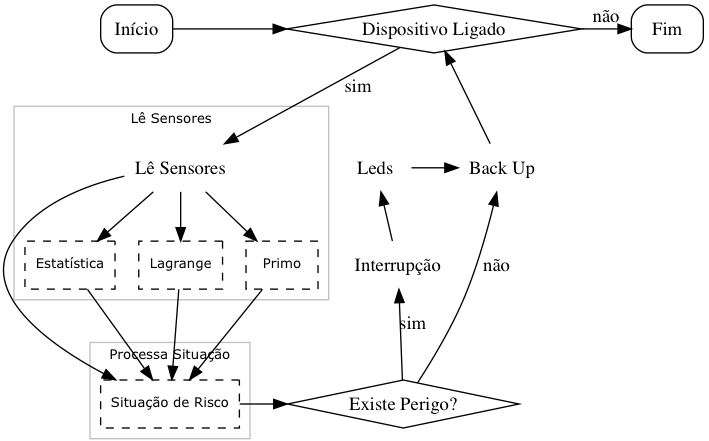
\includegraphics[width=0.48\textwidth]{img/capacete.png}
            \caption{Grafo de chamada do algoritmo base do \wearable. Itens quadriculados exibem a localização dos algoritmos candidatos ao particionamento.}
            \label{fig:gc}
        \end{figure}
        
        O particionamento foi avaliado em duas seções principais, sendo elas a de leitura e de processo de situações, constituindo-se de quatro situações diferentes de particionamento para análise (itens pontilhados na Figura \ref{fig:gc}).
        
        Os algoritmos \A$_{i}$\ candidatos ao particionamento serão:
        
        \begin{itemize}
            \item \A$_{Es}$: Análise Estatística (Algoritmo \ref{alg:statistic}) calculará valores de desvio padrão e variância dos valores no \buffer;
            
            \item \A$_{La}$: Lagrange (Algoritmo \ref{alg:lagrange}) interpolará novas distâncias a partir dos dados do \buffer; 
            \item \A$_{NP}$: Números Primos (Algoritmo \ref{alg:prime}) avaliará se a soma das distâncias lidas correspondem aos números primos;
            %As análises serão feitas por meio de exclusão, selecionando apenas um algoritmo por vez;
            \item \A$_{Ri}$: Processamento de risco (Algoritmo \ref{alg:risk}), na seção de processo de situações.
        \end{itemize}
    
    
        %!TEX root = ../main.tex
% !TeX encoding = UTF-8

       \begin{algorithm}[t] \footnotesize
           \KwIn{vetor buffer.}
           \KwOut{média, variância, desvio padrão.}
           
           \BlankLine
           \Begin{
               $\vars{soma}= \vars{variancia} = 0$;
               \BlankLine
               
               \lFor{$\func{length}(\vars{buffer})$}{$\vars{soma} \mathrel{+}= \vars{buffer}_i$}
               \BlankLine
               
               $\vars{media} = \vars{soma} \div \func{length}(\vars{buffer})$\;
               \BlankLine
               
               
               \lFor{$\func{length}(\vars{buffer})$}{
                   $\vars{variancia} \mathrel{+}= (\vars{buffer}_i - \vars{media})^2$
               }
               
               \BlankLine
               $\vars{variancia} \mathrel{\div}= \func{length}(\vars{buffer})$\;
               \BlankLine
               $\vars{dp} = \func{sqrt}(\vars{variancia})$\;
               
               \Return \vars{media}, \vars{variancia}, \vars{dp}\;
           }
           \caption{Método Estatístico.}
           \label{alg:statistic}
       \end{algorithm}
       
       \begin{algorithm}[b] \footnotesize
           \KwIn{vetor buffer, ponto.}
           \KwOut{distância interpolada.}
           
           \BlankLine
           \Begin{
               
               $\vars{nova\_distancia} = 0$\;
               \BlankLine
               
               \For{$\vars{i}\ in\ 1:\func{length}(\vars{buffer})$}{
                   $\vars{c} = \vars{d} = 1$;
                   
                   \BlankLine
                   \For{$\vars{j}\ in\ 1:\func{length}(\vars{buffer})$}{
                       \If{$\vars{i} \ne \vars{j}$}{
                           $\vars{c} \mathrel{\times}= \vars{ponto} - \vars{j}$;
                           %\BlankLine
                           $\vars{d} \mathrel{\times}= \vars{i} - \vars{j}$;
                       }
                   }
                   \BlankLine
                   $\vars{nova\_distancia} \mathrel{+}= \vars{buffer}_i \times \vars{c} \div \vars{d}$;
               }
               \BlankLine
               
               \lIf{$\vars{nova\_distancia} \ge 0$}{$\Return\ \vars{nova\_distancia}$}
               \lElse{$\Return\ 0$}
               
           }
           \caption{Método Interpolação por Lagrange.}
           \label{alg:lagrange}
       \end{algorithm}
       
       \begin{algorithm}[t] \footnotesize
           \KwIn{distância$_1$, distância$_2 = 0$, distância$_3 = 0$.}
           \KwOut{primaridade.}
           
           \BlankLine
           \Begin{
               
               $\vars{primo} = \vars{distancia}_1 + \vars{distancia}_2 + \vars{distancia}_3$;
               \BlankLine
               
               \lIf{$\vars{primo} \le 1$}{\Return 0}
               \BlankLine
               \lIf{$\vars{primo} = 2$}{\Return 1}
               \BlankLine
               
               \lIf{\vars{primo} $\func{mod}(2) = 0$}{$\vars{primo} \mathrel{+}= 1$}
               \BlankLine
               
               $\vars{divisor} = \vars{primo} \div 2$;
               
               \lIf{\vars{divisor} $\func{mod}(2) = 0$}{$\vars{divisor} \mathrel{+}= 1$}
               \BlankLine
               
               
               \While{\vars{divisor} $> 2$}{
                   \lIf{\vars{primo} $\func{mod}(divisor) = 0$}{\Return 0}
                   \BlankLine
                   \lElse{\vars{divisor} $\mathrel{-}= 2$;}
                   
               }
               \Return 1;
               
           }
           \caption{Método Número Primo.}
           \label{alg:prime}
       \end{algorithm}
       
       \begin{algorithm}[b]
           \footnotesize
           \KwIn{distância lida; distância mínima.}
           \KwOut{boolean.}
           
           \BlankLine
           \Begin{
               \tcp{Se há risco, retorna TRUE}
               \uIf{\vars{distancia\_lida} $\le$ \vars{distancia\_minima}}{
                   \Return 1
               }
               \lElse {
                   \Return 0
               }
               
           }
           \caption{Método avaliação de Risco.}
           \label{alg:risk}
       \end{algorithm}
       
        
        %Explicando as implementações de A
        Foi realizado o particionamento para cada algoritmo candidato \A$_{i}$, gerando tanto sua versão em código em nível de \software,\ quando seu módulo em \hardware,\ utilizados para testes comparativos de desempenho.
        
        % s de forma geral
        Para a execução dos testes, todos os \A$ _i $\ em suas versões \hs\ foram executados em implementações sistêmicas sintetizáveis \Ss$ _j $,\ constituídas de módulos como \textit{soft-}processador MicroBlaze, além de memórias, interfaces para comunicação com os dispositivos conectados, entre outros, permitindo o funcionamento completo do \wearable\ \cite{obeidat2011microblaze}.
        
        % as versões de a em software
        Todos os algoritmos \A$_{i}$ em suas versões de \software\ foram executados em uma única implementação \Ss$ _j $, já que esta era compatível com qualquer aplicação em nível de \software, dependendo somente da disposição das instruções na memória.
        Ou seja, para trocar o \A$_{i}$ por \A$_{k}$ neste sistema basta recompilar o projeto em \software.
        Os testes neste sistema serão referenciados como \Ss$ _{s} $.
        
        % algoritmos em hardwares
        % explicando que a necessitam de interfaces
        Algoritmos \A$ _i $\ em \hardware\ também executam em sistemas \Ss$ _j $, mas tais sistemas possuem características ímpares já que são acrescentados módulos sintetizáveis de cada algoritmo.
        %
        Como cada \A$_i$ possui seu próprio módulo, definiu-se um sistema \Ss$_j$ para cada algoritmo \A$_{i}$ em sua versão em nível de \hardware.
        
        Assim, como a Tabela~\ref{tab:bate_o_olho} exibe, \Ss$_s$ é o sistema para testes de todos os algoritmos \A$_{i}$\ em \softwares,\ não possuindo nenhuma adição de implementação sintetizável de \hardwares\ particionados.
        Os outros sistemas são para testes dos módulos dos respectivos algoritmos \A$ _i $ juntos de sua interface de comunicação \hs.
        
%        Dessa forma, os sistemas \Ss$_{j}$ que serão utilizados para teste são:
%        \begin{itemize}
%            \item \Ss$_s$: sistema para testes de todos os algoritmos \A$_{i}$\ em \softwares.
%            Não possui nenhuma adição de implementação sintetizável de \hardwares\ particionados;
%            \item \Ss$_{Es}$: sistema para testes do particionamento em \hardware\ do algoritmo \A$_{Es}$. 
%            Constitui-se do sistema acrescido do módulo sintetizável em \hardware\ \A$_{Es}$ e sua interface de comunicação com o módulo;
%            \item \Ss$_{La}$: sistema para testes do particionamento em \hardware\ do algoritmo \A$_{La}$. 
%            Constitui-se do sistema acrescido do módulo sintetizável em \hardware\ \A$_{La}$ e sua interface de comunicação com o módulo;
%            \item \Ss$_{NP}$: sistema para testes do particionamento em \hardware\ do algoritmo \A$_{NP}$. 
%            Constitui-se do sistema acrescido do módulo sintetizável em \hardware\ \A$_{NP}$ e sua interface de comunicação com o módulo; e
%            \item \Ss$_{Ri}$: sistema para testes do particionamento em \hardware\ do algoritmo \A$_{Ri}$. 
%            Constitui-se do sistema acrescido do módulo sintetizável em \hardware\ \A$_{Ri}$ e sua interface de comunicação com o módulo;
%        \end{itemize}
        
        \begin{table}[h]\centering
            \vspace{-1em}
            \scriptsize
            %\raaa{1.0}
            \raaa{0.9}
            \caption{Exibição dos Algoritmos Candidatos e os seus Sistemas para Teste}

\begin{tabular}{p{2.3em}p{1.3em}|p{1.3em}p{0.01em}p{1.3em}|p{1.3em}p{0.01em}p{1.3em}|p{1.3em}p{0.01em}p{1.3em}|p{1.3em}}
    \toprule
    & \multicolumn{2}{c}{\A$_{Es}$} && \multicolumn{2}{c}{\A$_{La}$} && \multicolumn{2}{c}{\A$_{NP}$} && \multicolumn{2}{c}{\A$_{Ri}$}\\ %\cmidrule{2-9}
    \cmidrule{2-3} \cmidrule{5-6} \cmidrule{8-9} \cmidrule{11-12}
    Impl.: & \textit{Soft.} & \textit{Hard.} && \textit{Soft.} & \textit{Hard.} && \textit{Soft.} & \textit{Hard.} && \textit{Soft.} & \textit{Hard.} \\ \midrule
    \Ss$_{s}$   & X &   && X &   && X &   && X &   \\ \hline
    \Ss$_{Es}$  &   & X &&   &   &&   &   &&   &   \\ \hline
    \Ss$_{La}$  &   &   &&   & X &&   &   &&   &   \\ \hline
    \Ss$_{NP}$  &   &   &&   &   &&   & X &&   &   \\ \hline
    \Ss$_{Ri}$  &   &   &&   &   &&   &   &&   & X \\
    \bottomrule
\end{tabular}
\label{tab:bate_o_olho}
\end{table}
        
        
        
        
    \subsubsection{Variações do Protótipo}
        A fim de fazer diferentes testes dos códigos particionados foi construído um protótipo modular para a realização de análises de desempenho sobre cada uma de suas variações.
        Os itens modulares são:
        \begin{itemize}
            \item Número de Sensores de Distância: testes serão realizados com um a três sensores. 
            Não aumenta-se a angulação de percepção, mas sim a exatidão dos dados lidos;
            \item \textit{Buffer} de Cada Sensor de Distância: \buffer\ de dados com tamanho 5, 10 e 15 para processamento das distâncias de cada sensor.
            Representam a quantidade de leituras que serão feitas para cada sensor, armazenando-as num vetor, na qual será utilizado como parâmetro para as operações que serão particionadas.
        \end{itemize}
        Dessa forma, sobre cada código candidato foi realizados testes segundo tais variações, tanto em \hardware,\ quanto em \software.
        %Além da avaliação de desempenho e gasto energético, é possível ter diferentes precisões de distância com tais variações.
        %algos
    
    
    \subsubsection{Equipamentos e Tecnologias Utilizadas}
        A placa utilizada para sintetização foi uma Arty A7-35T, com 32 mil \luts\ (LuTs) sem um \textit{hard-processor}, ou seja, um controlador/processador físico dedicado.
        Para isso, utilizou-se o sistema \textit{soft-processor} MicroBlaze para processamento do código em \software\ e comunicação com \hardware.
        
        
        Todos os algoritmos foram construídos utilizando-se a ferramenta HLS e incorporados ao projeto base com construções de circuitos digitais assistidos pelo computador.
        A comunicação entre \hs\ foi feita utilizando interface AXI.
        A medição de distância foi realizada com um sensor ultrassônico e a comunicação com um segundo dispositivo que utiliza \textit{Bluetooth Low Energy}.
        
        
    \subsection{Testes}
        % Explicando os testes
        Para a realização dos testes foi feito um procedimento, tendo como base a Figura \ref{fig:distance}. 
        Como o experimento foi realizado em laboratório, utilizou-se escala de centímetros para as análises.
        
        \begin{figure}[h] \centering
            %\vspace{-0.5em}
            
\includegraphics[width=0.5\textwidth]{img/distance.png}
            \caption{Simulação de aproximações de objetos perante o ciclista segundo suas respectivas áreas de segurança.}
            \label{fig:distance}
        \end{figure}
    
        Cada experimento foi realizado no decorrer de 12 iterações.
        Os principais passos do teste são:
        \begin{itemize}
            \item 
            %
            \textit{Iteração 1:} o ciclista, encontra-se a uma distância de 130 centímetros do objeto, sendo sua situação declarada como segura;
            %
            \item 
            \textit{Iteração 4:} o objeto inicia um movimento de aproximação\footnote{Tanto o movimento de aproximação quanto o de afastamento são realizados manualmente por humanos, simulando a situação real de um ciclista em seu meio.} ao ciclista chegando a ultrapassar o limite mínimo de 30 centímetros. Nisso, a situação do ciclista passa a ser de risco;
            %
            \item
            \textit{Iteração 6:} o objeto ainda encontra-se próximo ao ciclista;
            \item 
            \textit{Iteração 9:} o objeto afasta novamente do ciclista para 130 centímetros, retornando à situação segura;
            \item 
            \textit{Iteração 12:} última leitura para testes, ciclista ainda em situação segura.
            %
        \end{itemize}
    
        As iterações não citadas representam a permanência do estado da iteração anterior à ela.
   
        Este teste foi realizado em cada análise de particionamento com sua variação de módulo. 
        Ou seja, para cada um dos 4 algoritmos, em todas suas variações de sensores e \buffer, um total de 36 situações diferentes para \hs\ serão feitos 30 testes em sequência para cada uma dessas situações, para análises estatísticas de desempenho.
        
        Como a pesquisa tem o objetivo de avaliar o desempenho dos algoritmos candidatos em \hs,\ os tempos de envio de dados e atuação dos sensores foram descartados.
        
        \begin{comment}
        % filtros
        Para que fosse calculado o desempenho do sistema aplicou-se filtros dos quais eliminou-se os seguintes tempos: 
        \textit{a):} o tempo médio gasto da atuação dos sensores; bem como 
        \textit{b):} o tempo de envio para o dispositivo externo. 
        O motivo da filtragem é que o tempo de ambos depende diretamente da sua tecnologia 
        e isso interfere no tempo final.
        %
        Por exemplo, se em determinado teste o objeto ficar um pouco mais distante que 130 centímetros, o tempo da iteração completa será afetado, pois o cálculo depende diretamente da distância.
        O mesmo acontece com a comunicação sem fio, já que não ocorre em tempo constante e, caso falha reenvia-se a informação.
        
        Como o trabalho busca o estudo sobre o desempenho somente sobre a seção de código particionada, eliminou-se estes parâmetros de interferência dos resultados.
        %
        Dessa forma, os valores resultantes à desempenho são os tempos totais $\gamma =\ ^{software}\,/_{hardware} $ sem o tempo de atuação dos sensores e o tempo de envio ao dispositivo, tornando os resultados mais precisos sobre o particionamento.
        \end{comment}

        
\section{Resultados}   \label{chap:results}
    
    \subsection{Recursos Alocados para os Algoritmos \A$_{i}$ e Sistemas \Ss$_{j}$}
        %\todo[inline]{Nessa secao atual, a de testes, vc colocara merante uma tabela relacionado os Ss, Aalgoritmo, etc etc etc, de maneira q numa batida de olho de pra entender.}
        %\subsubsection{Recursos Para Cada Código Candidato \A}      
        
        % tabela hls
        Os valores exibidos pela Tabela \ref{tab:hls} quantificam os recursos utilizados pelo HLS para a geração de cada algoritmo \A$_{i}$ particionado em \hardware.
        %
        Cada linha exibe os valores de alocação referentes a cada algoritmo, sendo os algoritmos Estatístico \A$_{Es}$, Lagrange \A$_{La}$, Números Primos \A$_{NP}$ e Risco \A$_{Ri}$.
        %Já as colunas exibem para quais propósitos determinados recursos em \hardware\ foram utilizados, na qual expressões representam recursos em \hardware\ para cálculos lógico/matemáticos, instâncias para memorização de recursos utilizados nas expressões, assim como as alocações de multiplexadores e registradores para fins mais específicos\todo{melhorar}.
        Já as colunas exibem para quais propósitos determinados recursos em \hardware\ foram utilizados, na qual são expressões, instâncias, multiplexadores e registradores.
        Todos são formados das tecnologias \luts\ e \ffs.       
        %
        Na última coluna é contabilizado o total de gastos de cada \hardware\ gerado.
        
        \begin{table*}[t]\centering
            \vspace{-1em}
            \scriptsize
            %\raaa{1.0}
            \raaa{0.9}
            \caption{Recursos de FPGA Alocados para cada Código Particionado Utilizando HLS}
            \begin{tabular}{lrr|rr|rr|rr|rr}
                \toprule
                &\multicolumn{2}{c}{Expressões} & \multicolumn{2}{c}{Instâncias}      & \multicolumn{2}{c}{Multiplexadores}  & \multicolumn{2}{c}{Registradores} & \multicolumn{2}{c}{\textit{Total}} \\
                \cmidrule{2-11}
                %\cmidrule{2-3} \cmidrule{5-6} \cmidrule{8-9} \cmidrule{11-12} \cmidrule{14-15}
                & \luts & \ffs & \luts & \ffs & \luts & \ffs & \luts & \ffs & \luts & \ffs \\
                \midrule
                \A$_{Es}$&52 & 0     & 1948 & 1474   & 364 & 0      & 0 & 394   & 2364 & 1868 \\ 
                \A$_{La}$&128 & 0    & 2048 & 1425   & 309 & 0      & 0 & 479   & 2483 & 1904 \\ 
                \A$_{NP}$&1826 & 0   & 486 & 552     & 236 & 0      & 0 & 527   & 2448 & 1079 \\ 
                \A$_{Ri}$&18 & 0     & 120  & 82     & 15  & 0      & 0 & 34    & 153  & 116  \\ 
                \bottomrule
            \end{tabular}
            \label{tab:hls}
        \end{table*}
        
        %Linkando a com b
        %Com cada o módulo particionado gerado, deve-se então adicioná-los aos respectivos sistemas.
        
        
        
        %\subsubsection{Recursos Para Cada Sistema \Ss}
        
        Exibido os valores para cada \A$ _i $,\ a Tabela~\ref{tab:vivado} mostra os valores de alocação e gasto energético sobre cada sistema \Ss$_{j}$ utilizado para teste.
        As colunas exibem informações de alocação de \luts, \ffs\ e \luts RAM e o gasto energético médio (\textit{Chip Power}) de cada um dos sistemas \wearables\ testados no protótipo.
        A primeira linha exibe a quantidade de cada recurso disponível pela plataforma FPGA utilizada e as demais o valor alocado segundo cada sistema.
        
        \begin{table}[t]\centering
            \vspace{-1em}
            %\scriptsize
            \footnotesize 
            %\raaa{1.0}
            \raaa{0.9}
            \caption{Recursos e Gastos Energéticos Utilizados em todos os Sistemas Completos}
            \begin{tabular}{lcccc}
                \toprule
                & \lut   & Lu.T.\textit{RAM} & \ff             & \textit{Chip Power} \\
                \cmidrule{2-5}
                
                \textit{Disponível}& \textit{20800}  & \textit{9600}              & \textit{210}     & -      \\\cmidrule{1-5}
                \Ss$_{s}$ & 11991  & 1781              & 11612           & 0,922W \\
                \Ss$_{Es}$& 13640  & 1822              & 13080           & 0,972W \\ 
                \Ss$_{La}$& 13502  & 1808              & 13193           & 0,968W \\ 
                \Ss$_{NP}$& 12959  & 1782              & 12559           & 0,933W \\
                \Ss$_{Ri}$& 12109  & 1781              & 11742           & 0,929W \\ 
                \bottomrule
            \end{tabular}
            \label{tab:vivado}
        \end{table}
    
        Com esses valores é possível fazer análises de recursos utilizados tanto para os módulos de maneira isolada, quanto para o sistema como um todo.
        Assim, percebeu-se que:


   %\subsection{Análise sobre Quantidade de Recursos Alocados e Gasto Energético}
        %Analisando as Tabelas~\ref{tab:hls} e \ref{tab:vivado}, é possível ver que:
        
        \begin{itemize}
            \item 
            % codigo que gastou mais recurso
            \A$_{La}$ é o módulo particionado que utiliza mais recursos dentre todos.
            %Utilizou $8,1\%$ e $4,5\%$ do total disponível pela plataforma FPGA, sendo $18,3\%$ de \lut\ e $14,4\%$ de \ff\ do projeto final;
            Mesmo assim, ao incorporar os códigos particionados aos sistemas, seu sistema (\Ss$_{La}$) não é o maior em utilização de recursos;
            
            \item
            %sistema que mais gastou recursos
            Ainda sobre a utilização de recursos, a maior diferença entre sistemas completos (particionados com o sistema em \software)\ é de $5,5\%$, entre \Ss$_{s}$ e \Ss$_{Es}$. 
            Isso pois, enquanto o \Ss$_{s}$ utilizou $45,3\%$ do total de \luts\ disponíveis (ambas \luts\ e \luts RAM), \Ss$_{Es}$ utilizou $50,8\%$.
            
            Essa diferença entre recursos alocados também está presente na forma em que a interface de comunicação está sendo utilizada em seus módulos.
            Mesmo \A$_{Es}$ não sendo o maior módulo, seu sistema \Ss$_{Es}$ foi, indicando que sua interface requisitou grande quantia de recursos;
            
            \item
            Comparando o gasto energético dos sistemas particionados com o sistema em \software, o maior gasto também é de \Ss$_{Es}$, necessitando de $5,4\%$ W a mais que \Ss$_{s}$. \\
            O sistema com o módulo Lagrange em \hardware\ (\Ss$_{La}$) teve a menor diferença, utilizando $0,7\%$ Watts a mais que \Ss$_{s}$.
        \end{itemize}
           
           

    \subsection{Desempenho}
    
        A Figura \ref{fig:performance} exibe os valores obtidos das análise de desempenho entre \hs\ (conforme apresentado na Seção \ref{sec:ganho_performance}).
        Mostra-se todos os algoritmos separados em quadros, bem como suas variações de sensores e \buffer.
        
        No eixo das abscissas tem-se \textit{Sen} e \textit{Buf} representando a variação de sensores e do tamanho de \buffer\ no protótipo.
        Já no eixo das ordenadas exibe-se o valor performático dos 30 testes para cada uma das 36 situações, segundo a Equação~\ref{eq:speedup1}.
        
        \begin{figure*}[h] \centering
            \vspace{-0.5em}
            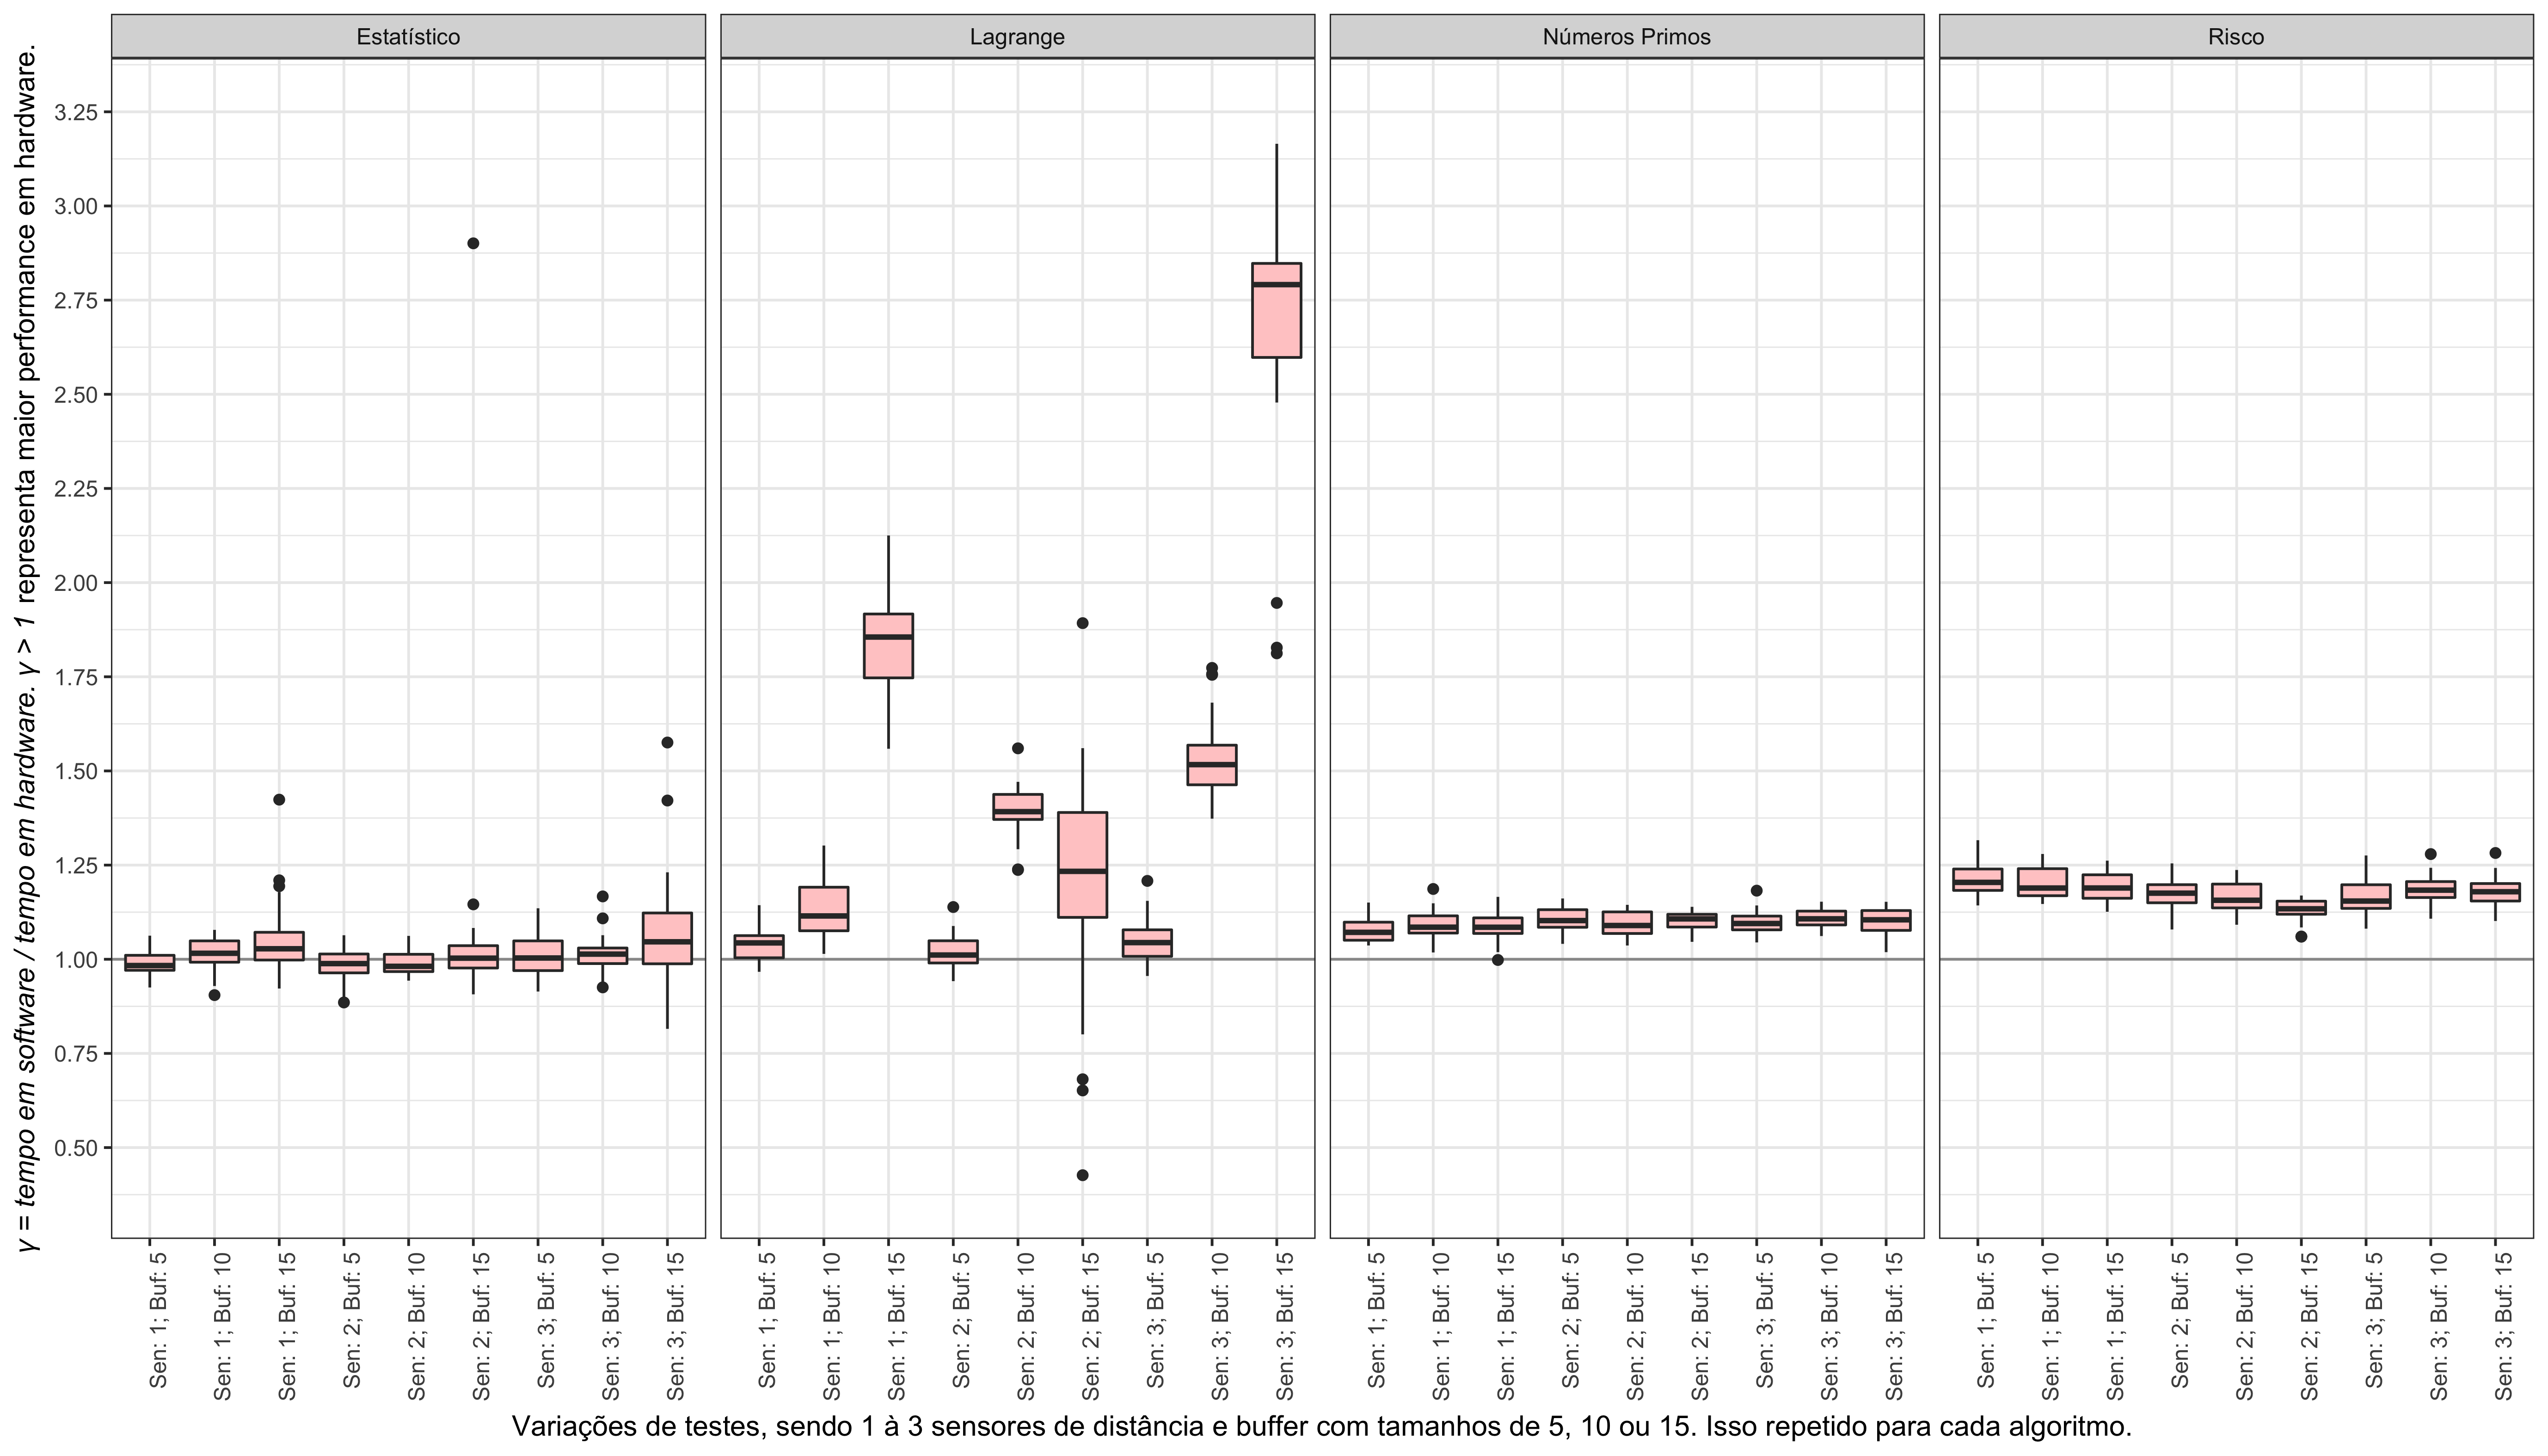
\includegraphics[width=1\textwidth]{img/performance.png}
            \caption{Gráfico com os valores performáticos de uma das 36 variações de protótipo, separados por código candidato. Valores de $\gamma > 1.0 $ exibem maior desempenho no \hardware\ particionado.}
            \label{fig:performance}
        \end{figure*}
   
    
        Além da Figura~\ref{fig:performance}, os valores médios também podem ser lidos pela Tabela~\ref{tab:performance}.
        Cada linha desta representa um quadro da Figura~\ref{fig:performance}.
        Como complemento, na última coluna tem-se uma média de desempenho de cada algoritmo em todas as suas variações de teste.
        
        \begin{table}[b]\centering
            \vspace{-1em}
            \scriptsize
            \raaa{1.0}
            %\raaa{0.9}
            \caption{Médias das Análises Performáticas em suas Variações}
            \begin{tabular}{@{}R{1.3em}R{1.6em}R{1.5em}R{1.5em}|R{1.6em}R{1.6em}R{1.6em}|R{1.5em}R{1.5em}R{1.5em}|c@{}}\toprule
                & \multicolumn{3}{c}{1 Sensor} & \multicolumn{3}{c}{2 Sensores} & \multicolumn{3}{c}{3 Sensores}& \\
                \cmidrule{2-11}
                \textit{Buffer} & 5 & 10 & 15 & 5 & 10 & 15 & 5 & 10 & 15 & $\bar{x}$ \\
                \midrule
                \Ss$_{Es}$   & 0.989 & 1.013 & 1.052  & 0.982 & 0.992 & 1.069  & 1.009 & 1.011 & 1.08  & 1.022 \\
                \Ss$_{La}$   & 1.036 & 1.132 & 1.844  & 1.019 & 1.395 & 1.14   & 1.046 & 1.37  & 2.765 & 1.416 \\
                \Ss$_{NP}$   & 1.076 & 1.092 & 1.084  & 1.105 & 1.094 & 1.103  & 1.099 & 1.109 & 1.102 & 1.096 \\ 
                \Ss$_{Ri}$   & 1.212 & 1.203 & 1.195  & 1.17  & 1.161 & 1.132  & 1.168 & 1.183 & 1.179 & 1.178 \\
                \bottomrule
            \end{tabular}
            \label{tab:performance}
        \end{table}
        
        %Análise de performance
        % quase todos foram suuuuuuuucesssooooooooo 
        Os resultados mostram que:
        \begin{itemize}
            \item 
            Os algoritmos Número Primo e Risco (\Ss$_{NP}$ e \Ss$_{Ri}$) obtiveram um ganho de desempenho considerável e estável, comparado com suas versões não particionadas, sendo em média $9,6\%$ e $17,8\%$ mais eficiente em suas tarefas;
            
            \item 
            Mesmo com o algoritmo Lagrange (\Ss$_{La}$) exibindo resultados não-estáveis nas variações como os de \Ss$_{NP}$ e \Ss$_{Ri}$, $87\%$ dos testes realizados obtiveram maior desempenho em \hardware.
            Superando a versão em \software\ em $41,6\%$;
            
            \item 
            O algoritmo Estatístico (\Ss$_{Es}$) obteve três situações, na qual não utilizar o particionamento resultava em maior desempenho, sendo $45,5\%$ foram iguais ou melhores em \software.
            %são (1; 5), (2; 5) e (2; 10) sendo números de sensores e tamanho de \buffer\ respectivamente.
            São elas: [\textit{Sen} 1; \textit{Buf} 5], [\textit{Sen} 2; \textit{Buf} 5] e [\textit{Sen} 2; \textit{Buf} 10]. 
            Entretanto, a média de todos os seus testes mostram que ainda assim foi $2,2\%$ mais eficiente em \hardware\ que \software.
        \end{itemize}
    
    
        %\item 
        % Achismos
        O baixo resultado de \Ss$_{Es}$ já era esperado, pois este e todos os outros algoritmos não receberam nenhuma otimização em \hardware,\ nem em sua interface de comunicação.
        O algoritmo Estático especificamente (Algoritmo \ref{alg:statistic}), é o único que realiza mais de uma leitura sobre os dados de \buffer\ via parâmetro, sendo as operações situadas nas linhas 3 e 5.
        Este algoritmo é custoso, pois o uso de cada elemento de \buffer\ requer também uma comunicação entre \hs,\ solicitando o respectivo dado, criando uma sobrecarga no barramento e, consequentemente, a queda de desempenho pela sua espera.
        
        %resolvendo o problema
        Este problema pode ser contornado de várias formas.
        A mais simples seria utilizar uma memória interna no \hardware\ extra que, após a cópia de todos os valores do \buffer, pode-se operar lendo da sua própria memória.
        \textit{Pipeline}, \textit{unroll} de \textit{loops} e protocolos de comunicação adequados são tipos de otimizações mais complexas, mas que poderiam resultar em melhora de desempenho, não aplicando só ao Estatístico, mas também todos os outros.
        
        
\begin{comment}


\begin{table}[h]\centering
\vspace{-1em}
\scriptsize
%\raaa{1.0}
\raaa{0.9}
\caption{Diferença Performática entre os Particionamentos par cada Conjunto de 12 Iterações do Wearable}
\begin{tabular}{@{}R{1.3em}R{1.6em}R{1.5em}R{1.5em}|R{1.6em}R{1.6em}R{1.6em}|R{1.5em}R{1.5em}R{1.5em}|c@{}}\toprule
& \multicolumn{3}{c}{1 Sensor} & \multicolumn{3}{c}{2 Sensores} & \multicolumn{3}{c}{3 Sensores}& \\
\cmidrule{2-11}
\textit{Buf} & 5 & 10 & 15 & 5 & 10 & 15 & 5 & 10 & 15 & $\bar{x}$ \\
\midrule
\Ss$_{Es}$   & -2.0   &    0.5  &    0.4  &   -2.7  &   -1.6  &   -1.8  &    0.4  &   0.3   &     4.2   & -0.2 \\
\Ss$_{La}$   &  7.7   &    9.3  &    8.6  &   10.9  &    9.9  &   11.6  &   10.2  &   12.0  &    12.1   & 10.2 \\
\Ss$_{NP}$   &  2.8   &   12.2  &   91.8  &    1.6  &   44.6  &   13.9  &    4.1  &   64.8  &   231.3   & 51.9 \\
\Ss$_{Ri}$   & 17.8   &   17.2  &   16.9  &   15.0  &   14.9  &   12.9  &   15.0  &   17.5  &    18.4   & 16.1 \\
\bottomrule
\end{tabular}
\label{tab:iterationsmilissegundos}
\end{table}


Power bigger  5,4229934924
Power little  0,7592190889

hls1 ao todo lt 7,7763157895
hls1 ao todo ff 4,4903846154

hls1 ao projeto lt 17,3313782991
hls1 ao projeto ff 14,2813455657

hls2 ao todo lt 8,1677631579
hls2 ao todo ff 4,5769230769

hls2 ao projeto lt 18,3898681677
hls2 ao projeto ff 14,4318957023

maior projeto lut 65,5769230769  ram 18,9791666667      lut all 50,8618421053    ff 31,7139423077             chip
software lut 57,6490384615       ram 18,5520833333      lut all 45,3026315789    ff 27,9134615385             chip

    Expression & Instance      & Multiplexer  & Register & Total
    52 / 0     & 1948 / 1474   & 364 / 0      & 0 / 394   & 2364 / 1868 \\ statistic
    128 / 0    & 2048 / 1425   & 309 / 0      & 0 / 479   & 2483 / 1904 \\ lagrange
    1826 / 0   & 486 / 552     & 236 / 0      & 0 / 527   & 2448 / 1079 \\ prime
    18 / 0     & 120  / 82     & 15  / 0      & 0 / 34    & 153  / 116  \\ risk
    
    
    & LUT    & LUTRAM   & FF     & IO     & On-Chip Power & Power supplied to off-chip devices
    & 20800  & 9600     & 41600  & 210    & -             & - \\
    & 13640  & 1822     & 13080  & 104    & 0,972         & 0,506 \\ statistic
    & 13502  & 1808     & 13193  & 104    & 0,968         & 0,506 \\ lagrange
    & 12959  & 1782     & 12559  & 104    & 0,933         & 0,506 \\ prime
    & 12109  & 1781     & 11742  & 104    & 0,929         & 0,506 \\ risk
    
    (-2,0   +    0,5  +    0,4  +   -2,7  +   -1,6  +   -1,8  +    0,4  +   0,3   +     4,2) / 9 = -0.2
    ( 7,7   +    9,3  +    8,6  +   10,9  +    9,9  +   11,6  +   10,2  +   12,0  +    12,1) / 9 = 10.2
    ( 2,8   +   12,2  +   91,8  +    1,6  +   44,6  +   13,9  +    4,1  +   64,8  +   231,3) / 9 = 51.9
    (17,8   +   17,2  +   16,9  +   15,0  +   14,9  +   12,9  +   15,0  +   17,5  +    18,4) / 9 = 16.1
    
\end{comment}


\begin{comment}
    \begin{table}\centering
    \scriptsize
    \raaa{1.3}
    \caption{Cálculo de desempenho sobre variações em I/O e algoritmo particionado.}
    \begin{tabular}{@{}rrrrcrrrcrrr@{}}\toprule
    & \multicolumn{3}{c}{$\mathcal{O}(1)$} && \multicolumn{3}{c}{$\mathcal{O}(n)$} & & \multicolumn{3}{c}{$\mathcal{O}(n\log n)$}\\
    \cmidrule{2-4} \cmidrule{6-8} \cmidrule{10-12}análise& 5 & 10 & 15 && 5 & 10 & 15 &&5 & 10 & 15 \\
    \midrule \textit{sistêmica} \\
    %média     & ? & ? & ? && ? & ? & ? && ? & ? & ? \\
    $\bar{x}$     & ? & ? & ? && ? & ? & ? && ? & ? & ? \\
    $\sigma^2$ & ? & ? & ? && ? & ? & ? && ? & ? & ? \\
    $\sigma$ & ? & ? & ? && ? & ? & ? && ? & ? & ? \\
    \midrule \textit{empírica} \\
    %média     & ? & ? & ? && ? & ? & ? && ? & ? & ? \\
    $\bar{x}$     & ? & ? & ? && ? & ? & ? && ? & ? & ? \\
    $\sigma^2$ & ? & ? & ? && ? & ? & ? && ? & ? & ? \\
    $\sigma$ & ? & ? & ? && ? & ? & ? && ? & ? & ? \\
    \bottomrule
    \end{tabular}
    \end{table}
    \end{frame}
\end{comment}



%!TEX root = ../main.tex
% !TeX encoding = UTF-8
\section{Conclusões} \label{chap:conclu}
    %projeto de sistemas
    A demanda por curto tempo para disponibilidade ao mercado, somado ao fato dos produtos exigirem propriedades de corretude, rapidez, confiabilidade e preço acessível representam um desafio para projetistas de sistemas embarcados em geral.
    %utiliza o particionamento para o problema de desempenho
    Com o desenvolvimento de sistemas embarcados cada vez mais complexos, o particionamento \hs\ tornou-se um problema de otimização em \codesign\ de sistemas.
    %wearable
    Como dispositivos \wearables\ também demandam um alto desempenho e/ou baixo consumo de energia sem apresentar desequilíbrio em confiabilidade e segurança entre outros, aplicou-se o particionamento sobre essa classe de sistemas, com foco em tais melhorias.
    
    %proposta
    A proposta da pesquisa constituiu-se na busca pelo aprimoramento de desempenho de dispositivos computacionais \wearables,\ utilizando o particionamento como meio, visando gasto energético e de recursos limitados de plataforma FPGA.
    
    %comentando os testes
    Para a avaliação, realizou-se particionamento de quatro algoritmos candidatos (Estatístico \A$_{Es}$, Lagrange \A$_{La}$, Números Primos  \A$_{NP}$ e Processamento de Risco \A$_{Ri}$) de um projeto de capacete de segurança para ciclistas, variando cada teste em quantidade de sensores e também o \buffer\ de operação.
    
    % comentando os resultados
    Três dos quatro sistemas (Lagrange \Ss$_{La}$, Números Primos \Ss$_{NP}$ e Risco \Ss$_{Ri}$) obtiveram sucesso na busca por desempenho apenas pelo processo de particionamento, aumentando no mínimo $9,6\%$ seus desempenhos, utilizando o valor máximo de $ 5,5\% $ de recursos e $ 5,4\% $ de energia do \hardware\ reconfigurável.
    %
    O sistema Estatístico \Ss$_{Es}$ em $45,5\%$ dos testes obteve maior desempenho \software\ comparado com \hardware.
    Esse resultado já era esperado, já que seu código exige bastante comunicação entre \hs, afetando seu desempenho.

    %trabalhos futuros
    %har e softprocessadores
    Para futuros trabalhos seria possível realizar a comparação do sistema \wearable\ particionado variando, também a arquitetura de sintetização, ou seja, testes de desempenho entre \textit{soft} e \textit{hard-}processadores, ambos utilizando FPGA.
    
    % fpga e prototipações
    %Comparações entre o uso de plataformas FPGA e plataformas de prototipações também seriam viáveis, ainda com foco em busca em otimizações em desempenho e eficiência energética sobre \wearables.
    
    %mais alguma sugestão de trabalhos?
    %E também a adição do parâmetro otimização em \hardware,\ verificando o percentual de ganho ao utilizar as técnicas de otimizações em nível de \hardware\ existentes para HLS.
    
    
    % use section* for acknowledgment
    \section*{Agradecimentos}
        Agradecemos à Universidade Federal de Ouro Preto, ao CNPq, CAPES e à FAPEMIG pelo subsídio dessa pesquisa.        

   % conference papers do not normally have an appendix
   %\section*{Apêndice}    
   %    \hphantom{a}


\section*{Referências}

\begingroup
\renewcommand{\section}[2]{}
% can use a bibliography generated by BibTeX as a .bbl file
% BibTeX documentation can be easily obtained at:
% http://mirror.ctan.org/biblio/bibtex/contrib/doc/
% The IEEEtran BibTeX style support page is at:
% http://www.michaelshell.org/tex/ieeetran/bibtex/
\bibliographystyle{IEEEtran}
% argument is your BibTeX string definitions and bibliography database(s)
%\bibliography{bibliography}
\bibliography{IEEEabrv,bibliography}

\endgroup

\end{document}
